Poglavje vsebuje rezultate testiranj programa na zgoraj opisanih podatkovnih množicah po načrtu poglavja~\ref{sec:nacrt-poskusov}.
Rezultati so navedeni na naslednji način:
\begin{itemize}
    \item vsak podrazdelek zajema rezultate testiranja programa na določeni podatkovni množici,
    \item znotraj podrazdelka je navedena tabela z naborom inicializacijskih parametrov, katere bomo uporabili pri testiranju,
    \item sledijo ji dejanski rezultati za vsak nabor parametrov:
    \begin{itemize}
        \item tabela s točnostjo oz.\ MCC najboljših agentov vsakega od petih zagonov,
        \item matrika zmot najbolj točnega agenta in agenta z največjim MCC,
        \item graf točnosti in MCC populacije, kateri pripada najboljši agent, skozi generacije,
        \item vizualizacija najbolj točnega agenta in agenta z največjim MCC.
    \end{itemize}
\end{itemize}

\subsection{Iris}\label{subsec:iris_test}
%% arrowLength=4
%% linkWidth=5
%% input fy=100*node.pos
%% output fx=300
%% output fy=100*node.pos
%% MAX_FONT_SIZE=3
\begin{table}[H]
    \caption{Nabori inicializacijskih parametrov poganjanja na množici Iris.}
    \begin{center}
        \begin{tabular}{||l c c c||}
            \hline
            & 1      & 2      & 3 \\ [0.5ex]
            \hline
            velikost populacije               & 100    & 150    & 200    \\
            \hline
            največje število globokih vozlišč & 5      & 10     & 15     \\
            \hline
            največje število povezav          & 10     & 20     & 30     \\
            \hline
            največje število prečkanj         & 2      & 2      & 3      \\
            \hline
            delež mutiranih potomcev          & 10\%   & 10\%   & 10\%   \\
            \hline
            prispevek vozlišč                 & -0.001 & -0.001 & -0.001 \\
            \hline
            prispevek povezav                 & -0.001 & -0.001 & -0.001 \\
            \hline
            število generacij                 & 200    & 200    & 300    \\
            \hline
        \end{tabular}
    \end{center}
    \label{tab:param_iris}
\end{table}

\subsubsection{Prvi nabor}
%%"/home/jure/CLionProjects/Neuroevolution/datasets/iris/iris.data" 100 5 10 2 true 0.1 50 true -0.001 -0.001 500 ACC
\begin{table}[H]
    \caption{Rezultat prvega nabora parametrov.}
    \begin{center}
        \begin{tabular}{|| c | c c || c c ||}
            \hline
            \multirow{2}{*}{št. zagona} & \multicolumn{2}{c||}{točnost najboljšega agenta} & \multicolumn{2}{c||}{MCC najboljšega agenta} \\ \cline{2-5}
            & učna    & testna           & učna  & testna         \\
            \hline
            1        & 0.705\% & 0.578\%          & 0.609 & 0.617          \\
            \hline
            2        & 0.667\% & 0.667\%          & 0.633 & 0.567          \\
            \hline
            3        & 0.962\% & \textbf{0.889\%} & 0.673 & 0.698          \\
            \hline
            4        & 0.829\% & 0.733\%          & 0.601 & 0.632          \\
            \hline
            5        & 0.714\% & 0.756\%          & 0.9   & \textbf{0.800} \\
            \hline
            $\sigma$ & 0.108   & 0.105            & 0.111 & 0.08           \\
            \hline
        \end{tabular}
    \end{center}
    \label{tab:iris_result_1}
\end{table}

\begin{table}[H]
    \centering
    \caption{Matrika zmot najbolj točnega agenta prvega nabora.}
    \begin{tabular}{||rcccc||}
        \hline
        razred           & Iris Setosa & Iris Versicolour & Iris Virginica & vsota \\ \hline
        Iris Setosa      & 15          & 0                & 0              & 15    \\ \hline
        Iris Versicolour & 0           & 11               & 5              & 16    \\ \hline
        Iris Virginica   & 0           & 0                & 14             & 14    \\ \hline
        vsota            & 15          & 11               & 19             & 45    \\ \hline
    \end{tabular}
    \label{tab:iris_acc_1}
\end{table}

\begin{table}[H]
    \centering
    \caption{Matrika zmot agenta z največjim MCC prvega nabora.}
    \begin{tabular}{||rcccc||}
        \hline
        razred           & Iris Setosa & Iris Versicolour & Iris Virginica & vsota \\ \hline
        Iris Setosa      & 14          & 0                & 0              & 14    \\ \hline
        Iris Versicolour & 0           & 12               & 3              & 15    \\ \hline
        Iris Virginica   & 0           & 3                & 13             & 16    \\ \hline
        vsota            & 14          & 15               & 16             & 45    \\ \hline
    \end{tabular}
    \label{tab:iris_mcc_1}
\end{table}

\begin{figure}[H]
    \begin{center}
        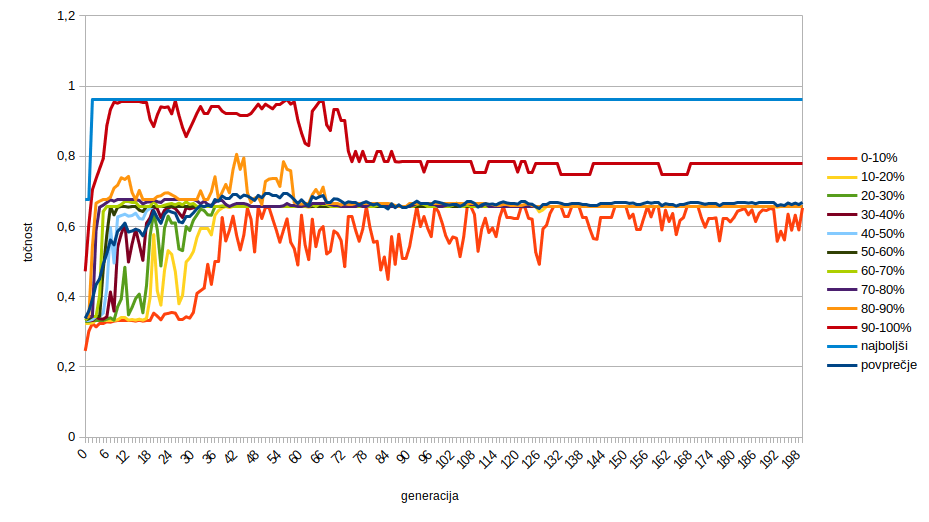
\includegraphics[width=13cm]{iris/1/acc}
    \end{center}
    \caption{Graf točnosti populacije najboljšega agenta prvega nabora skozi generacije.}
    \label{fig:iris_acc_1}
\end{figure}

\begin{figure}[H]
    \begin{center}
        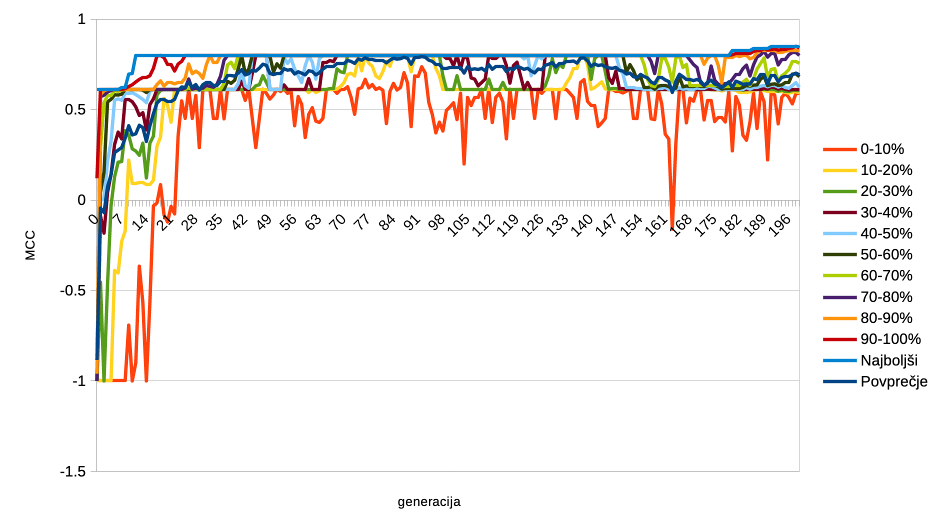
\includegraphics[width=13cm]{iris/1/mcc}
    \end{center}
    \caption{Graf MCC populacije najboljšega agenta prvega nabora skozi generacije.}
    \label{fig:iris_mcc_1}
\end{figure}

\begin{figure}[H]
    \begin{center}
        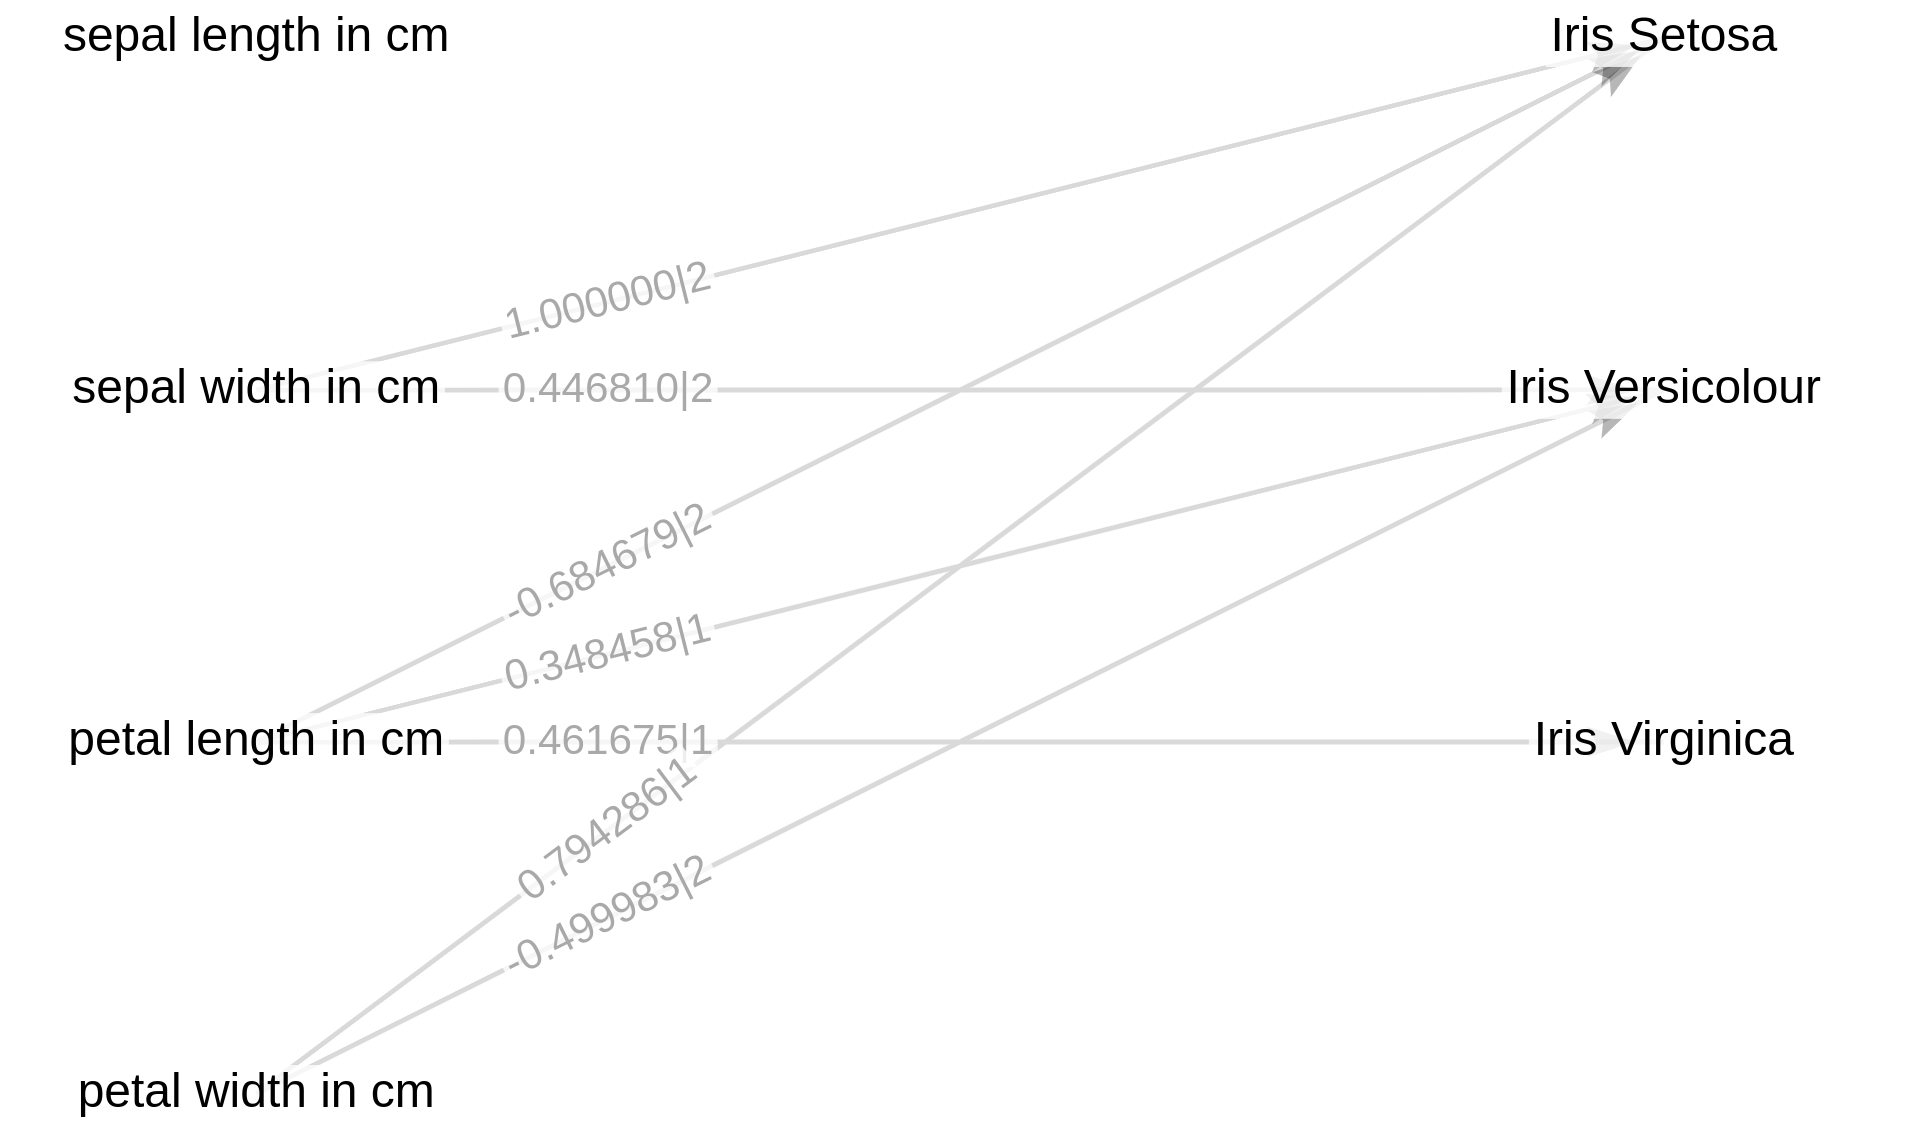
\includegraphics[width=13cm]{iris/1/acc_g}
    \end{center}
    \caption{Vizualizacija najbolj točnega agenta prvega nabora. Vsebuje 7 povezav.}
    \label{fig:iris_acc_1_g}
\end{figure}

\begin{figure}[H]
    \begin{center}
        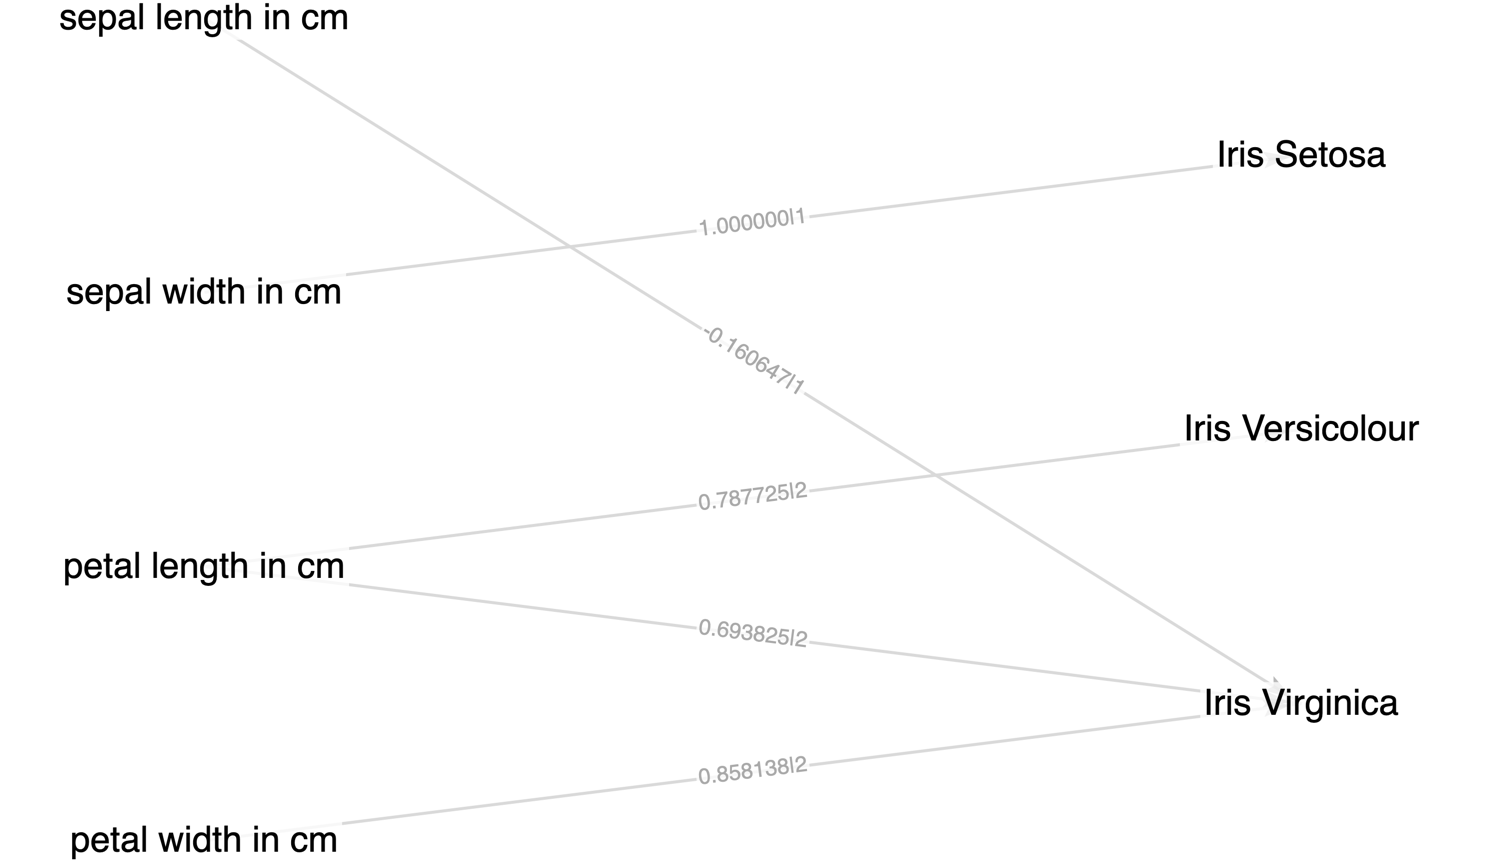
\includegraphics[width=13cm]{iris/1/mcc_g}
    \end{center}
    \caption{Vizualizacija agenta z največjim MCC prvega nabora. Vsebuje 1 globoko vozlišče in 8 povezav.}
    \label{fig:iris_mcc_1_g}
\end{figure}

\subsubsection{Drugi nabor}
%%"/home/jure/CLionProjects/Neuroevolution/datasets/iris/iris.data" 200 15 30 3 true 0.1 100 true -0.001 -0.001 200 ACC
\begin{table}[H]
    \caption{Rezultat drugega nabora parametrov.}
    \begin{center}
        \begin{tabular}{|| c | c c || c c ||}
            \hline
            \multirow{2}{*}{št. zagona} & \multicolumn{2}{c||}{točnost najboljšega agenta} & \multicolumn{2}{c||}{MCC najboljšega agenta} \\ \cline{2-5}
            & učna    & testna           & učna  & testna         \\
            \hline
            1        & 0.952\% & 0.956\%          & 0.93  & 0.906          \\
            \hline
            2        & 0.981\% & 0.867\%          & 0.634 & 0.561          \\
            \hline
            3        & 0.952\% & 0.933\%          & 0.944 & \textbf{0.967} \\
            \hline
            4        & 0.981\% & 0.889\%          & 0.888 & 0.837          \\
            \hline
            5        & 0.952\% & \textbf{0.978\%} & 0.929 & 0.906          \\
            \hline
            $\sigma$ & 0.014   & 0.041            & 0.117 & 0.143          \\
            \hline
        \end{tabular}
    \end{center}
    \label{tab:iris_result_2}
\end{table}

\begin{table}[H]
    \centering
    \caption{Matrika zmot najbolj točnega agenta drugega nabora.}
    \begin{tabular}{||rcccc||}
        \hline
        razred           & Iris Setosa & Iris Versicolour & Iris Virginica & vsota \\ \hline
        ris Setosa       & 15          & 0                & 0              & 15    \\ \hline
        Iris Versicolour & 0           & 17               & 0              & 17    \\ \hline
        Iris Virginica   & 0           & 1                & 12             & 13    \\ \hline
        vsota            & 15          & 18               & 12             & 45    \\ \hline
    \end{tabular}
    \label{tab:iris_acc_2}
\end{table}

\begin{table}[H]
    \centering
    \caption{Matrika zmot agenta z največjim MCC drugega nabora.}
    \begin{tabular}{||rcccc||}
        \hline
        razred           & Iris Setosa & Iris Versicolour & Iris Virginica & vsota \\ \hline
        ris Setosa       & 15          & 0                & 0              & 15    \\ \hline
        Iris Versicolour & 0           & 12               & 1              & 13    \\ \hline
        Iris Virginica   & 0           & 0                & 17             & 17    \\ \hline
        vsota            & 15          & 12               & 18             & 45    \\ \hline
    \end{tabular}
    \label{tab:iris_mcc_2}
\end{table}

\begin{figure}[H]
    \begin{center}
        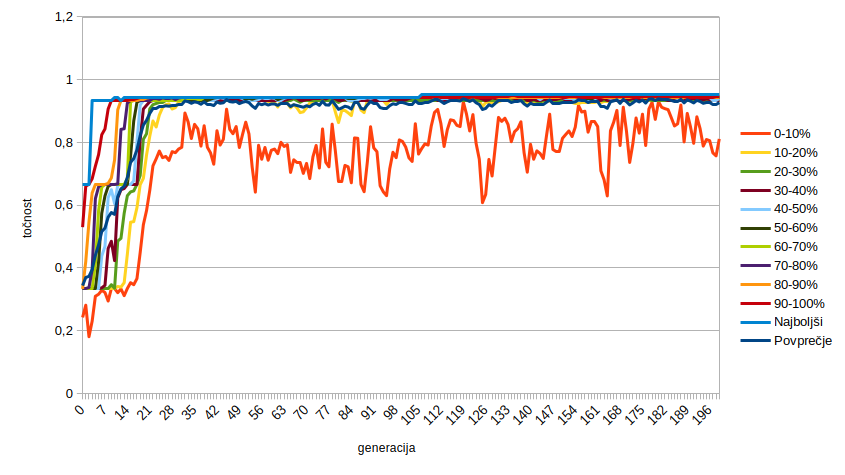
\includegraphics[width=13cm]{iris/2/acc}
    \end{center}
    \caption{Graf točnosti populacije najboljšega agenta drugega nabora skozi generacije.}
    \label{fig:iris_acc_2}
\end{figure}

\begin{figure}[H]
    \begin{center}
        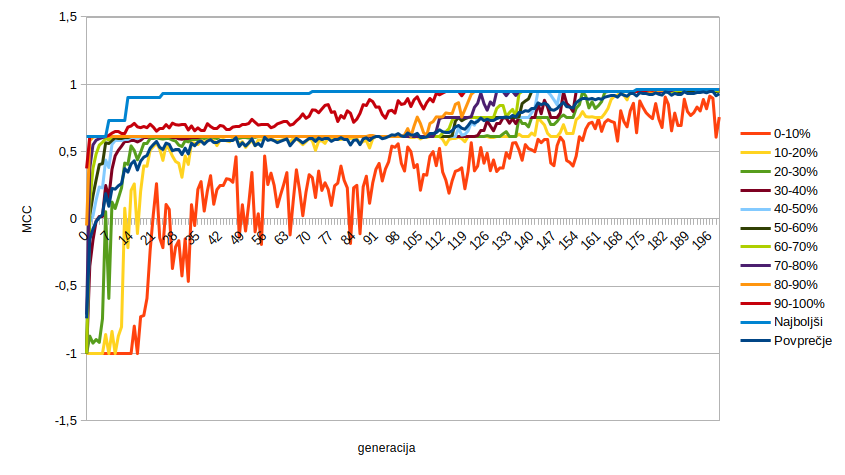
\includegraphics[width=13cm]{iris/2/mcc}
    \end{center}
    \caption{Graf MCC populacije najboljšega agenta drugega nabora skozi generacije.}
    \label{fig:iris_mcc_2}
\end{figure}

\begin{figure}[H]
    \begin{center}
        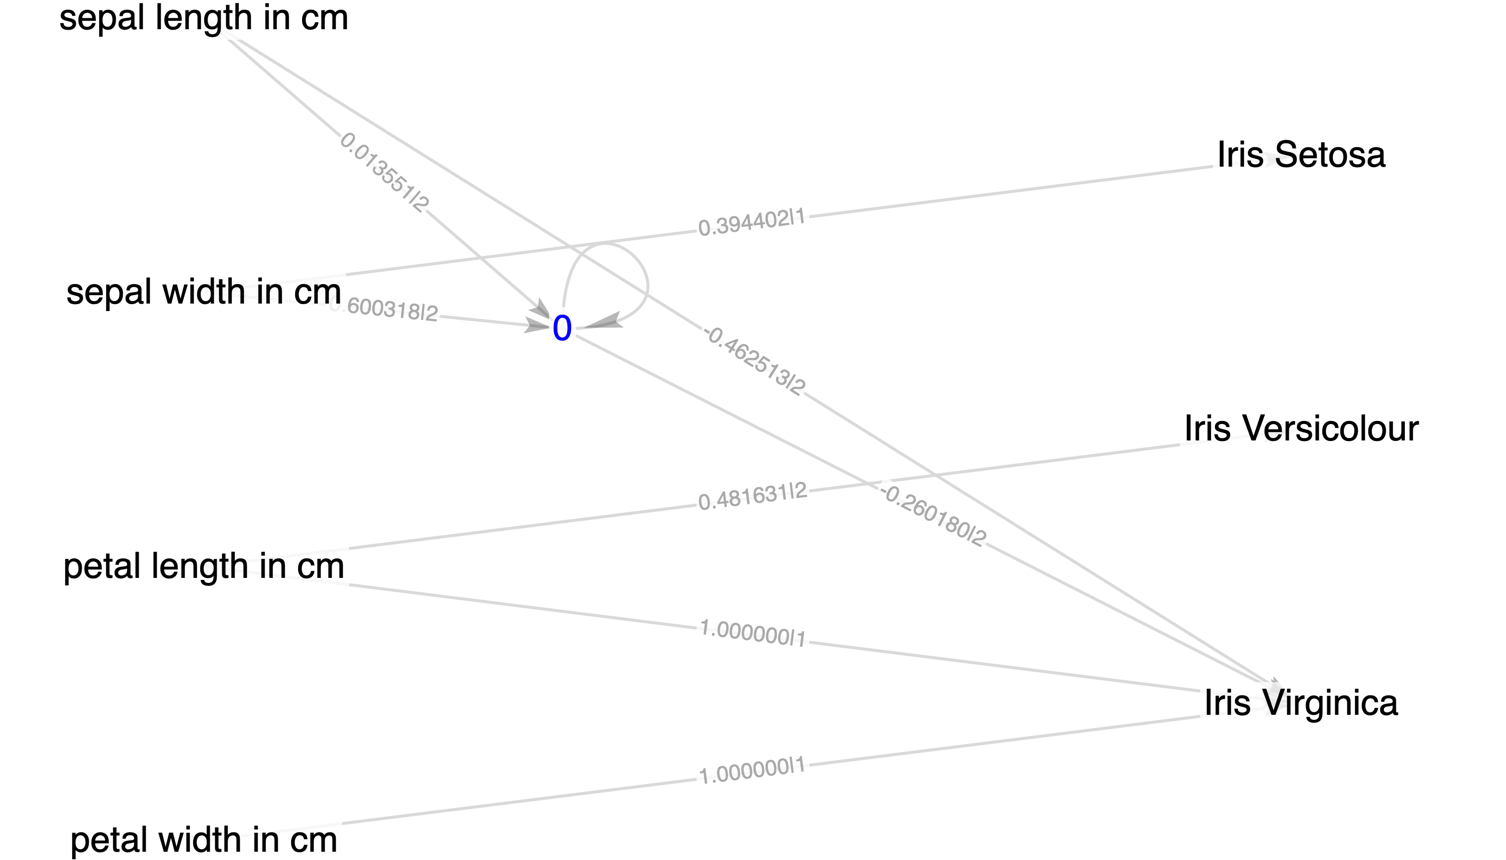
\includegraphics[width=13cm]{iris/2/acc_g}
    \end{center}
    \caption{Vizualizacija najbolj točnega agenta drugega nabora. Vsebuje 4 globoka vozlišča in 15 povezav.}
    \label{fig:iris_acc_2_g}
\end{figure}

\begin{figure}[H]
    \begin{center}
        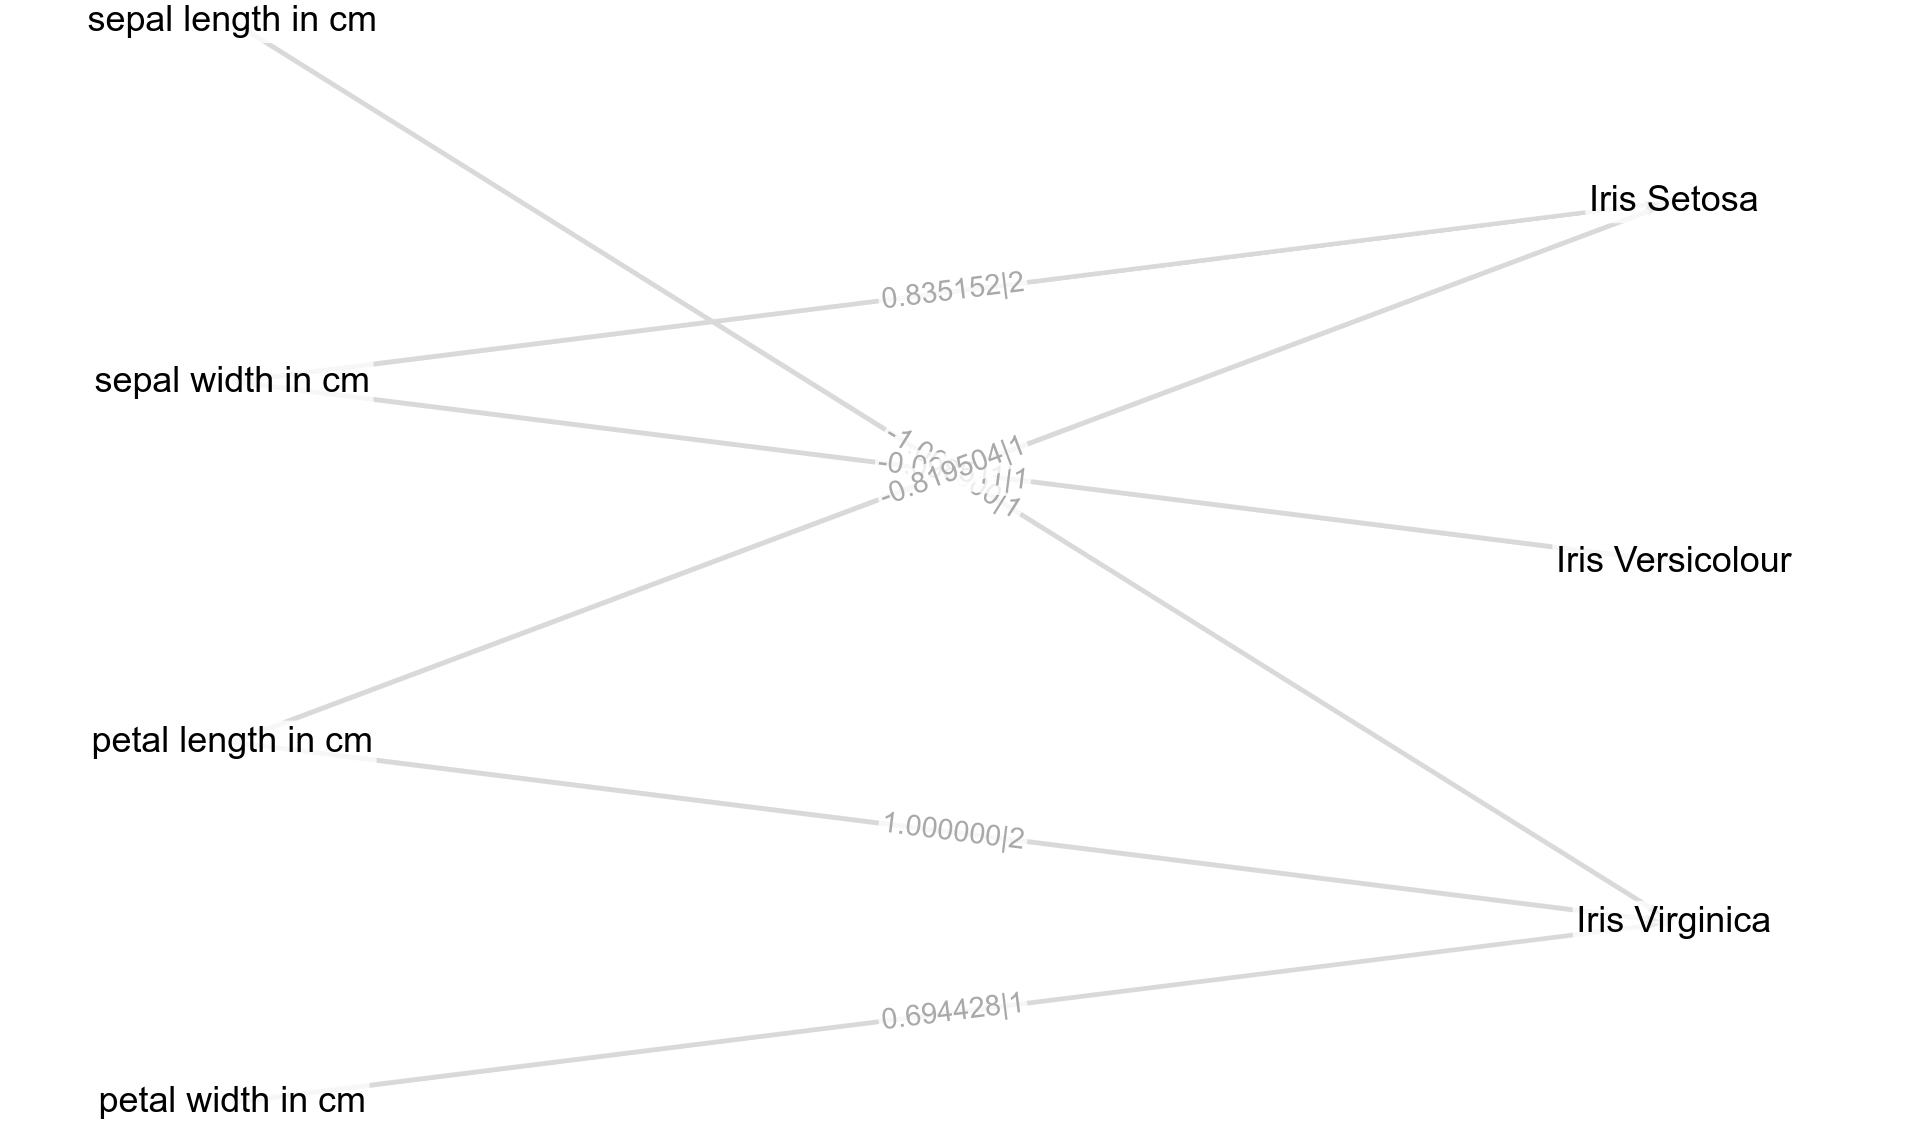
\includegraphics[width=13cm]{iris/2/mcc_g}
    \end{center}
    \caption{Vizualizacija agenta z največjim MCC drugega nabora. Vsebuje 3 globoka vozlišča in 12 povezav.}
    \label{fig:iris_mcc_2_g}
\end{figure}

\subsubsection{Tretji nabor}
%%"/home/jure/CLionProjects/Neuroevolution/datasets/iris/iris.data" 200 15 30 3 true 0.1 100 true -0.001 -0.001 300 ACC
\begin{table}[H]
    \caption{Rezultat tretjega nabora parametrov.}
    \begin{center}
        \begin{tabular}{|| c | c c || c c ||}
            \hline
            \multirow{2}{*}{št. zagona} & \multicolumn{2}{c||}{točnost najboljšega agenta} & \multicolumn{2}{c||}{MCC najboljšega agenta} \\ \cline{2-5}
            & učna    & testna           & učna  & testna         \\
            \hline
            1        & 0.971\% & 0.978\%          & 0.932 & 0.901          \\
            \hline
            2        & 0.962\% & 0.956\%          & 0.901 & \textbf{0.936} \\
            \hline
            3        & 0.962\% & \textbf{1.000\%} & 0.957 & 0.877          \\
            \hline
            4        & 0.981\% & 1.000\%          & 0.972 & 0.906          \\
            \hline
            5        & 0.971\% & 0.956\%          & 0.930 & 0.877          \\
            \hline
            $\sigma$ & 0.007   & 0.020            & 0.024 & 0.022          \\
            \hline
        \end{tabular}
    \end{center}
    \label{tab:iris_result_3}
\end{table}

\begin{table}[H]
    \centering
    \caption{Matrika zmot najbolj točnega agenta tretjega nabora (zagon 3).}
    \begin{tabular}{||rcccc||}
        \hline
        razred           & Iris Setosa & Iris Versicolour & Iris Virginica & vsota \\ \hline
        ris Setosa       & 15          & 0                & 0              & 15    \\ \hline
        Iris Versicolour & 0           & 15               & 0              & 15    \\ \hline
        Iris Virginica   & 0           & 0                & 15             & 15    \\ \hline
        vsota            & 15          & 15               & 15             & 45    \\ \hline
    \end{tabular}
    \label{tab:iris_acc_3}
\end{table}

\begin{table}[H]
    \centering
    \caption{Matrika zmot agenta z največjim MCC tretjega nabora.}
    \begin{tabular}{||rcccc||}
        \hline
        razred           & Iris Setosa & Iris Versicolour & Iris Virginica & vsota \\ \hline
        ris Setosa       & 15          & 0                & 0              & 15    \\ \hline
        Iris Versicolour & 0           & 15               & 0              & 15    \\ \hline
        Iris Virginica   & 0           & 2                & 13             & 15    \\ \hline
        vsota            & 15          & 17               & 13             & 45    \\ \hline
    \end{tabular}
    \label{tab:iris_mcc_3}
\end{table}

\begin{figure}[H]
    \begin{center}
        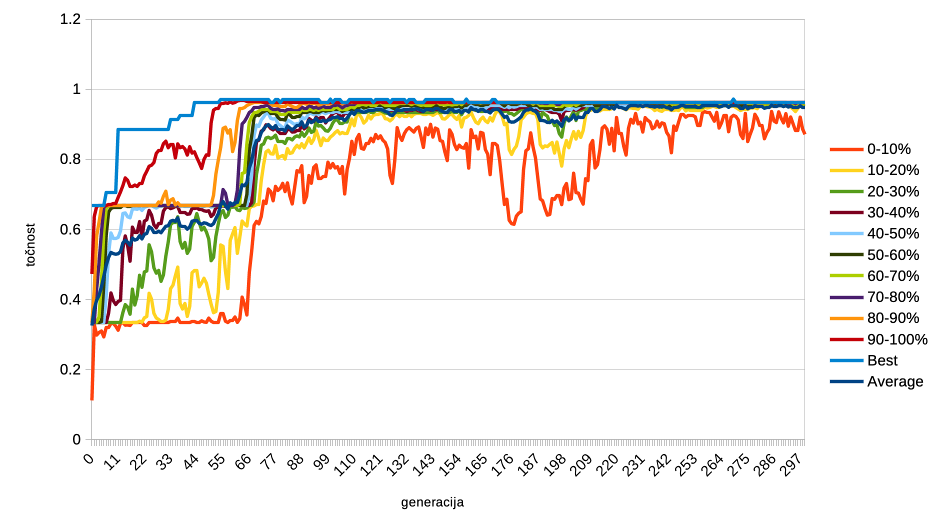
\includegraphics[width=13cm]{iris/3/acc}
    \end{center}
    \caption{Graf točnosti populacije najboljšega agenta tretjega nabora skozi generacije (zagon 3).}
    \label{fig:iris_acc_3}
\end{figure}

\begin{figure}[H]
    \begin{center}
        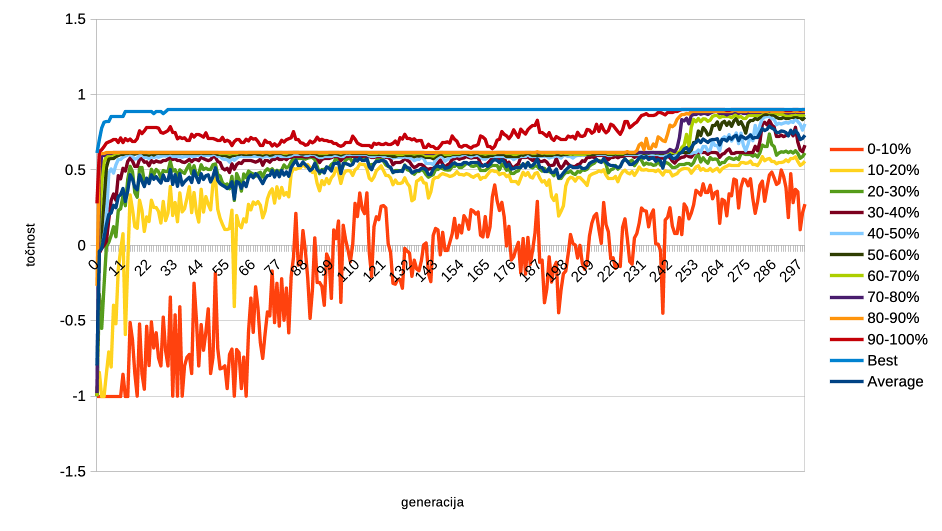
\includegraphics[width=13cm]{iris/3/mcc}
    \end{center}
    \caption{Graf MCC populacije najboljšega agenta tretjega nabora skozi generacije.}
    \label{fig:iris_mcc_3}
\end{figure}

\begin{figure}[H]
    \begin{center}
        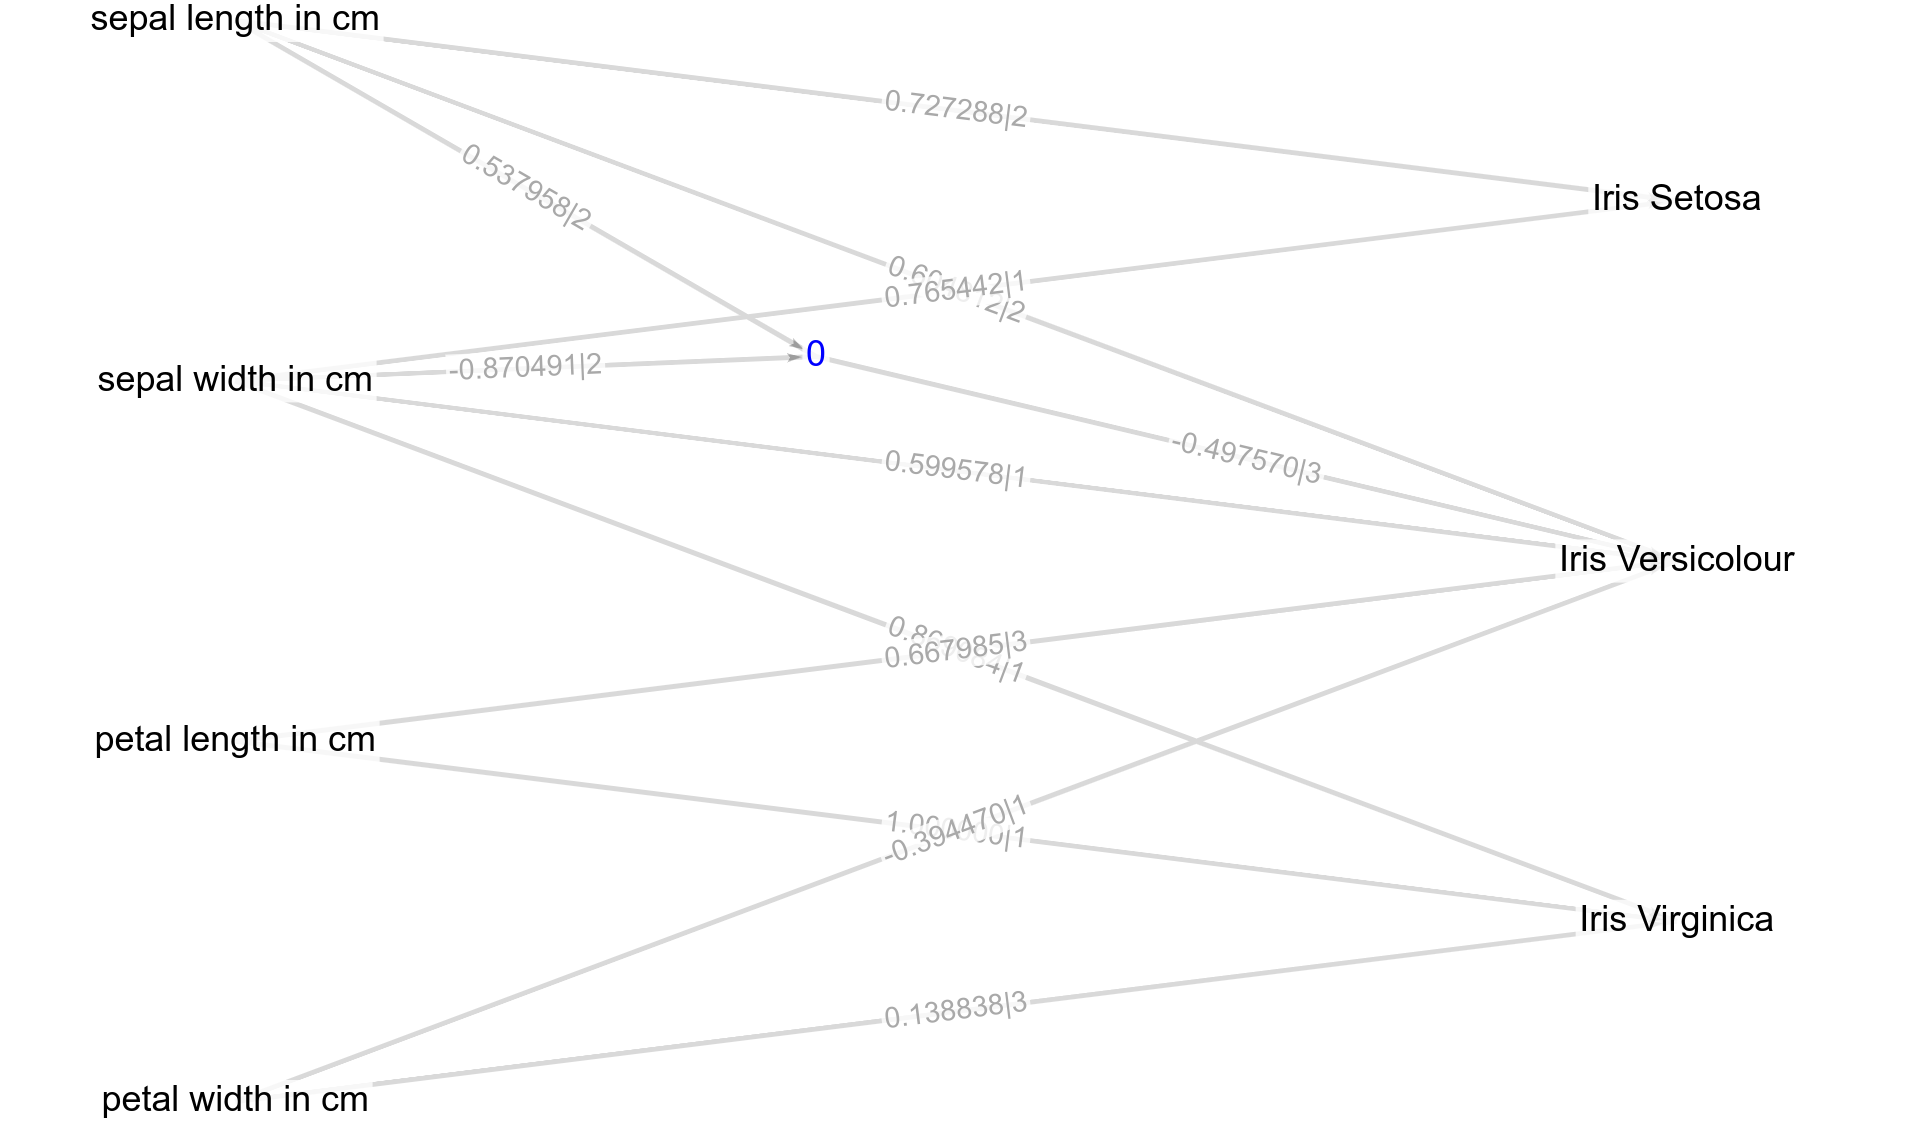
\includegraphics[width=13cm]{iris/3/acc_g}
    \end{center}
    \caption{Vizualizacija najbolj točnega agenta tretjega nabora (zagon 3). Vsebuje 2 globoka vozlišča in 10 povezav.}
    \label{fig:iris_acc_3_g}
\end{figure}

\begin{figure}[H]
    \begin{center}
        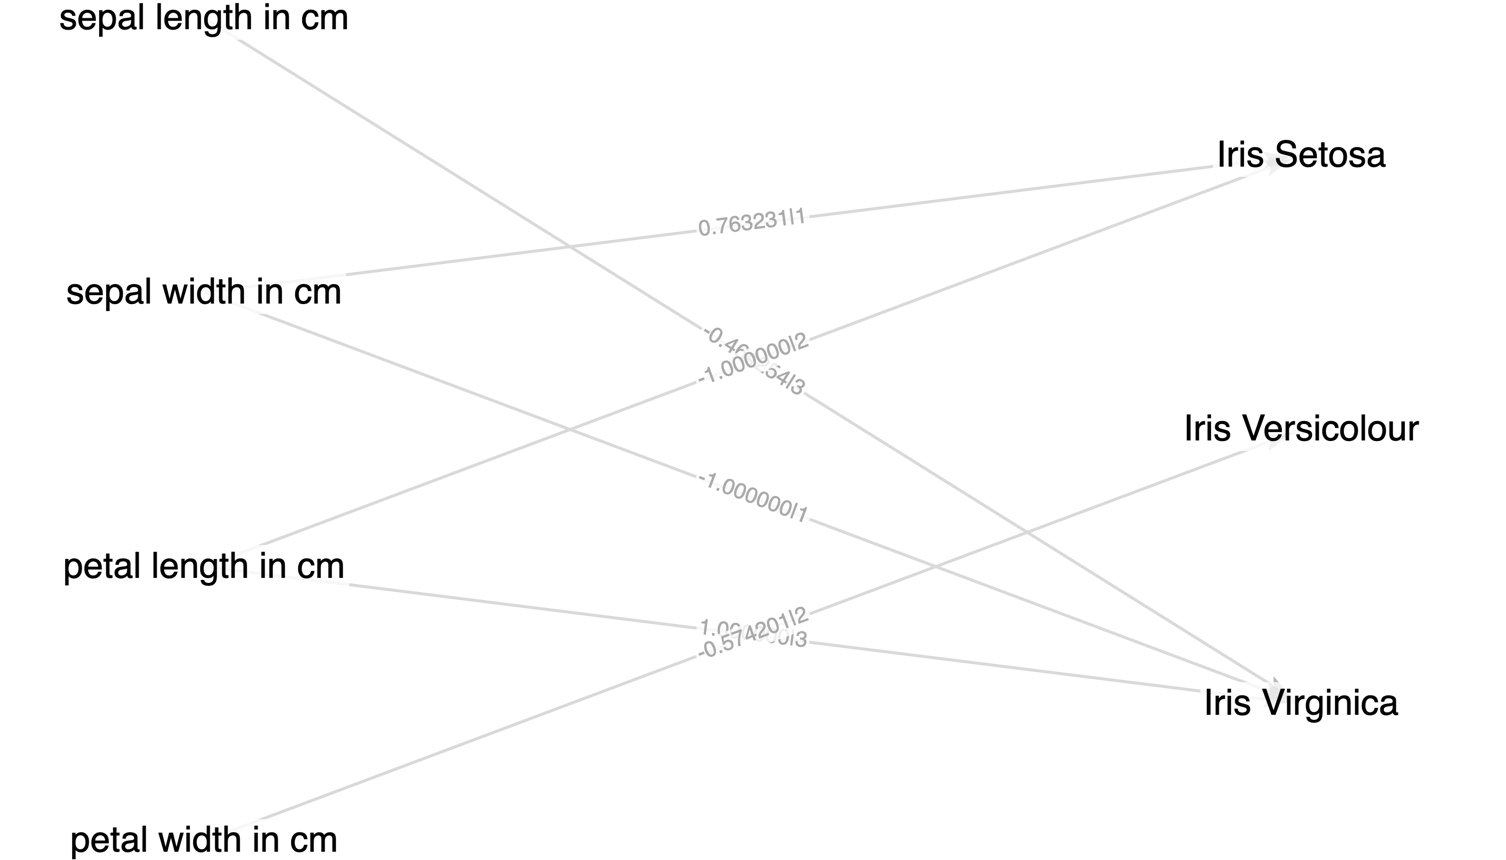
\includegraphics[width=13cm]{iris/3/mcc_g}
    \end{center}
    \caption{Vizualizacija agenta z največjim MCC drugega nabora. Vsebuje 6 globokih vozlišč in 23 povezav.}
    \label{fig:iris_mcc_3_g}
\end{figure}

\subsection{Wine}\label{subsec:wine_test}
%% arrowLength=20
%% linkWidth=2
%% input fy=50*node.pos
%% output fx=700
%% output fy=150*node.pos+120
%% MAX_FONT_SIZE=12
\begin{table}[H]
    \caption{Nabori inicializacijskih parametrov poganjanja na množici Wine.}
    \begin{center}
        \begin{tabular}{||l c c c||}
            \hline
            & 1      & 2      & 3 \\ [0.5ex]
            \hline
            velikost populacije               & 200    & 250    & 350    \\
            \hline
            največje število globokih vozlišč & 15     & 20     & 25     \\
            \hline
            največje število povezav          & 30     & 50     & 75     \\
            \hline
            največje število prečkanj         & 2      & 3      & 4      \\
            \hline
            delež mutiranih potomcev          & 10\%   & 10\%   & 10\%   \\
            \hline
            prispevek vozlišč                 & -0.001 & -0.001 & -0.001 \\
            \hline
            prispevek povezav                 & -0.001 & -0.001 & -0.001 \\
            \hline
            število generacij                 & 300    & 350    & 450    \\
            \hline
        \end{tabular}
    \end{center}
    \label{tab:param_wine}
\end{table}

\subsubsection{Prvi nabor}
%%"/home/jure/CLionProjects/Neuroevolution/datasets/wine/wine.data" 200 15 30 2 true 0.1 100 true -0.001 -0.001 300 ACC
\begin{table}[H]
    \caption{Rezultat prvega nabora parametrov.}
    \begin{center}
        \begin{tabular}{|| c | c c || c c ||}
            \hline
            \multirow{2}{*}{št. zagona} & \multicolumn{2}{c||}{točnost najboljšega agenta} & \multicolumn{2}{c||}{MCC najboljšega agenta} \\ \cline{2-5}
            & učna    & testna           & učna  & testna         \\
            \hline
            1        & 0.880\% & 0.830\%          & 0.874 & 0.755          \\
            \hline
            2        & 0.952\% & \textbf{0.962\%} & 0.904 & 0.720          \\
            \hline
            3        & 0.928\% & 0.868\%          & 0.939 & \textbf{0.943} \\
            \hline
            4        & 0.928\% & 0.906\%          & 0.699 & 0.721          \\
            \hline
            5        & 0.888\% & 0.887\%          & 0.869 & 0.860          \\
            \hline
            $\sigma$ & 0.027   & 0.044            & 0.034 & 0.088          \\
            \hline
        \end{tabular}
    \end{center}
    \label{tab:wine_result_1}
\end{table}

\begin{table}[H]
    \centering
    \caption{Matrika zmot najbolj točnega agenta prvega nabora.}
    \begin{tabular}{||rcccc||}
        \hline
        razred  & Class 1 & Class 2 & Class 3 & vsota \\ \hline
        Class 1 & 18      & 0       & 0       & 18    \\ \hline
        Class 2 & 0       & 19      & 2       & 21    \\ \hline
        Class 3 & 0       & 0       & 14      & 14    \\ \hline
        vsota   & 18      & 19      & 16      & 53    \\ \hline
    \end{tabular}
    \label{tab:wine_acc_1}
\end{table}

\begin{table}[H]
    \centering
    \caption{Matrika zmot agenta z največjim MCC prvega nabora.}
    \begin{tabular}{||rcccc||}
        \hline
        razred  & Class 1 & Class 2 & Class 3 & vsota \\ \hline
        Class 1 & 17      & 1       & 0       & 18    \\ \hline
        Class 2 & 1       & 20      & 0       & 21    \\ \hline
        Class 3 & 0       & 0       & 14      & 14    \\ \hline
        vsota   & 18      & 21      & 14      & 53    \\ \hline
    \end{tabular}
    \label{tab:wine_mcc_1}
\end{table}

\begin{figure}[H]
    \begin{center}
        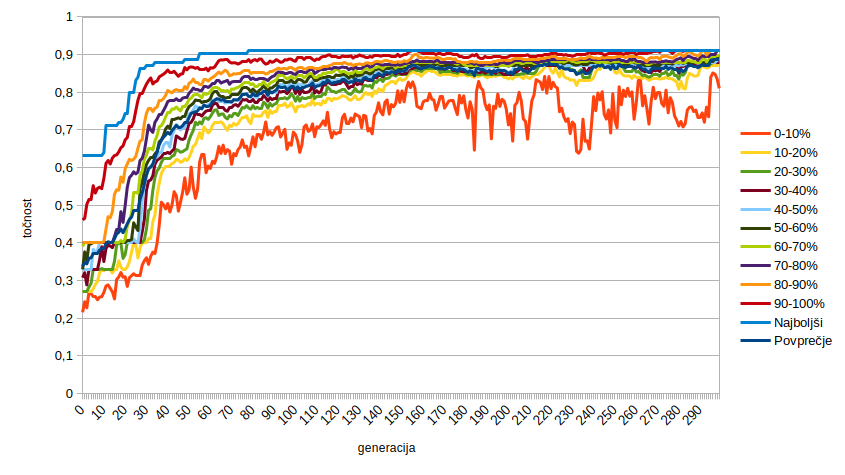
\includegraphics[width=13cm]{wine/1/acc}
    \end{center}
    \caption{Graf točnosti populacije najboljšega agenta prvega nabora skozi generacije.}
    \label{fig:wine_acc_1}
\end{figure}

\begin{figure}[H]
    \begin{center}
        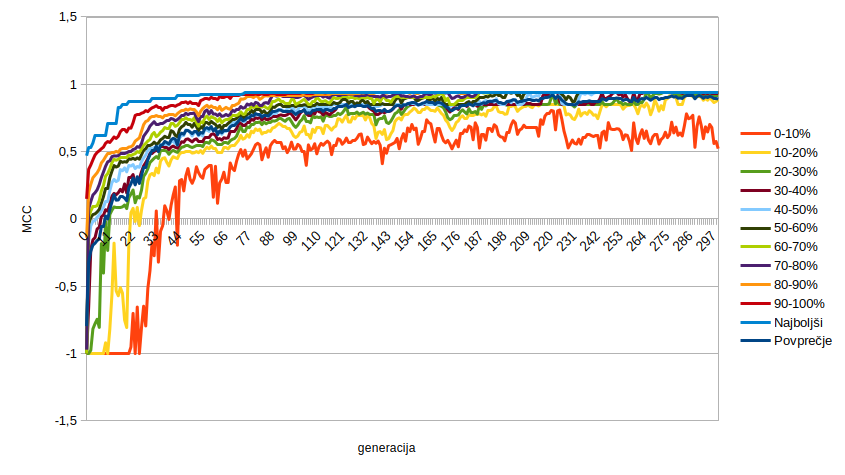
\includegraphics[width=13cm]{wine/1/mcc}
    \end{center}
    \caption{Graf MCC populacije najboljšega agenta prvega nabora skozi generacije.}
    \label{fig:wine_mcc_1}
\end{figure}

\begin{figure}[H]
    \begin{center}
        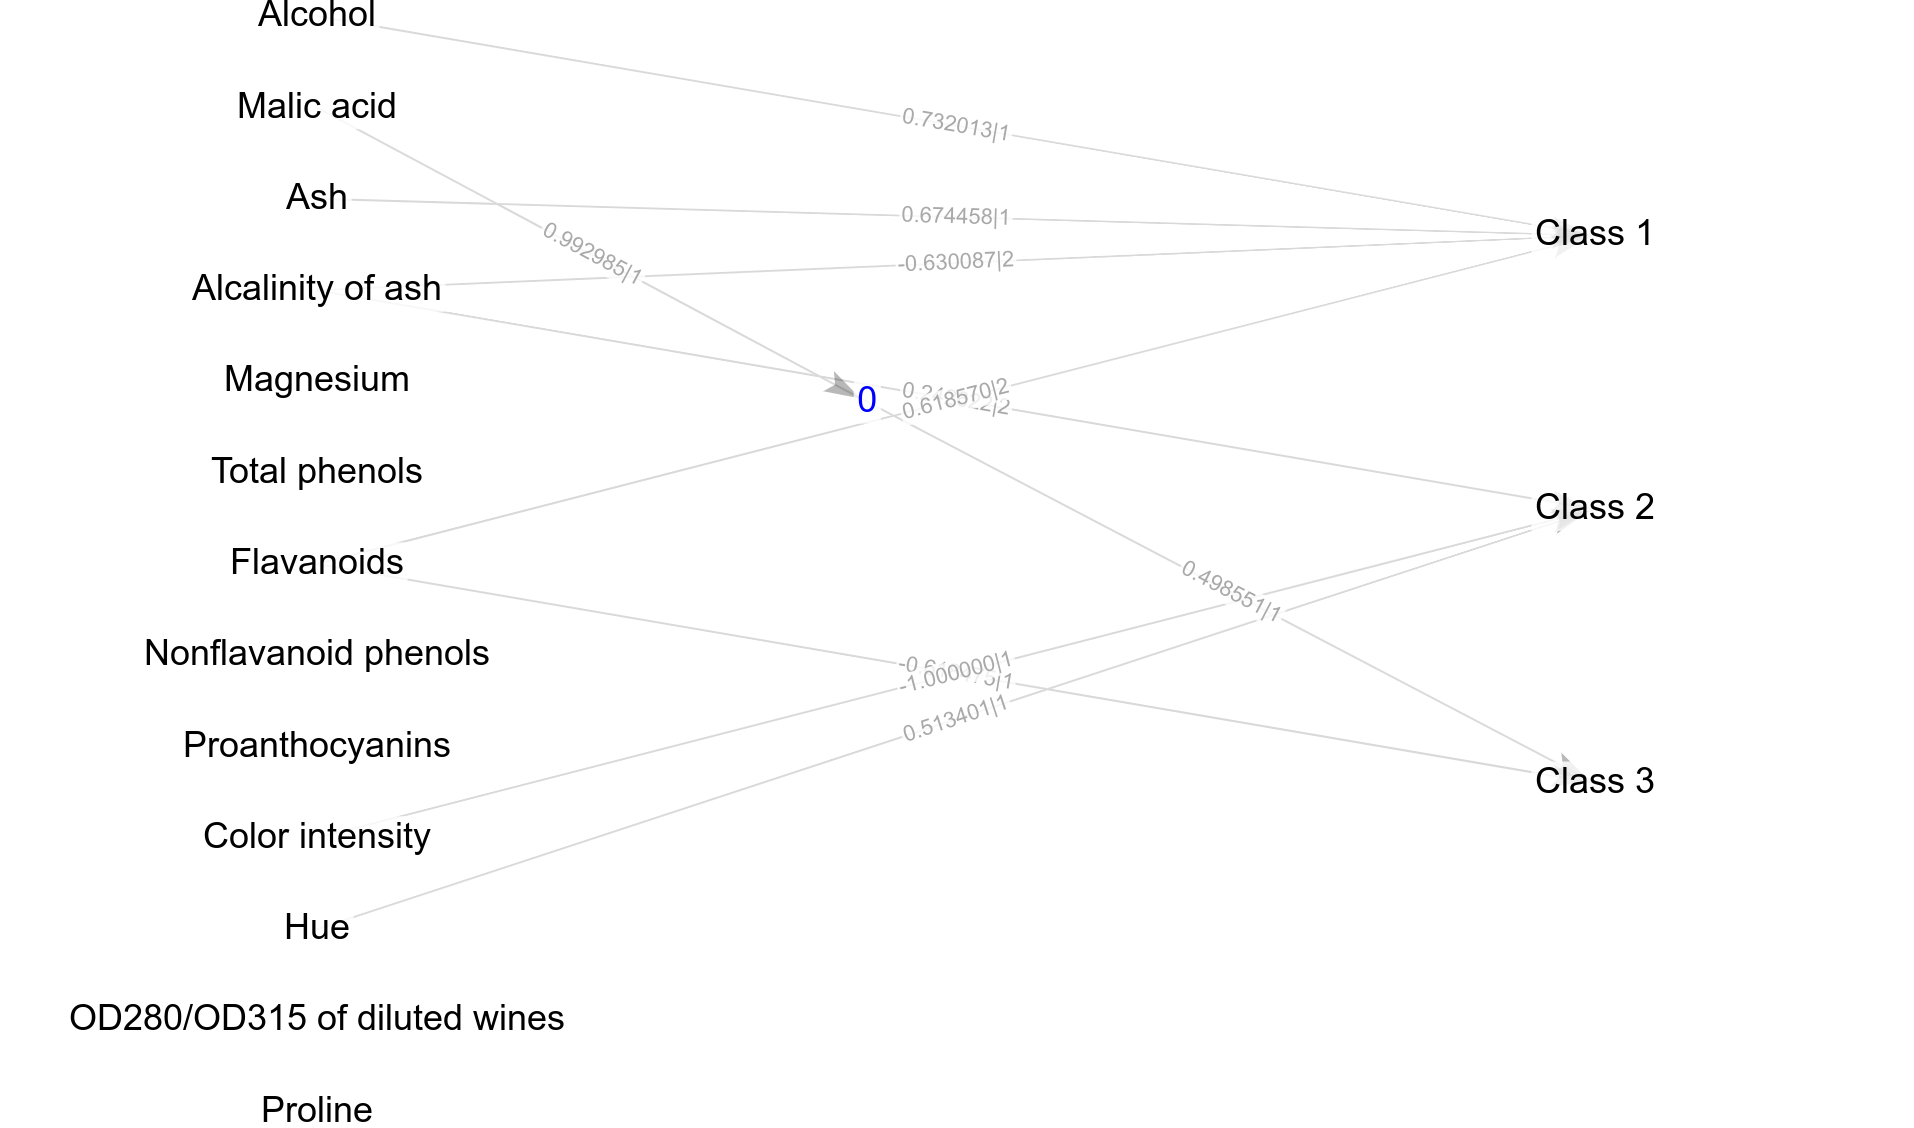
\includegraphics[width=13cm]{wine/1/acc_g}
    \end{center}
    \caption{Vizualizacija najbolj točnega agenta prvega nabora. Vsebuje 4 globoka vozlišča in 23 povezav.}
    \label{fig:wine_acc_1_g}
\end{figure}

\begin{figure}[H]
    \begin{center}
        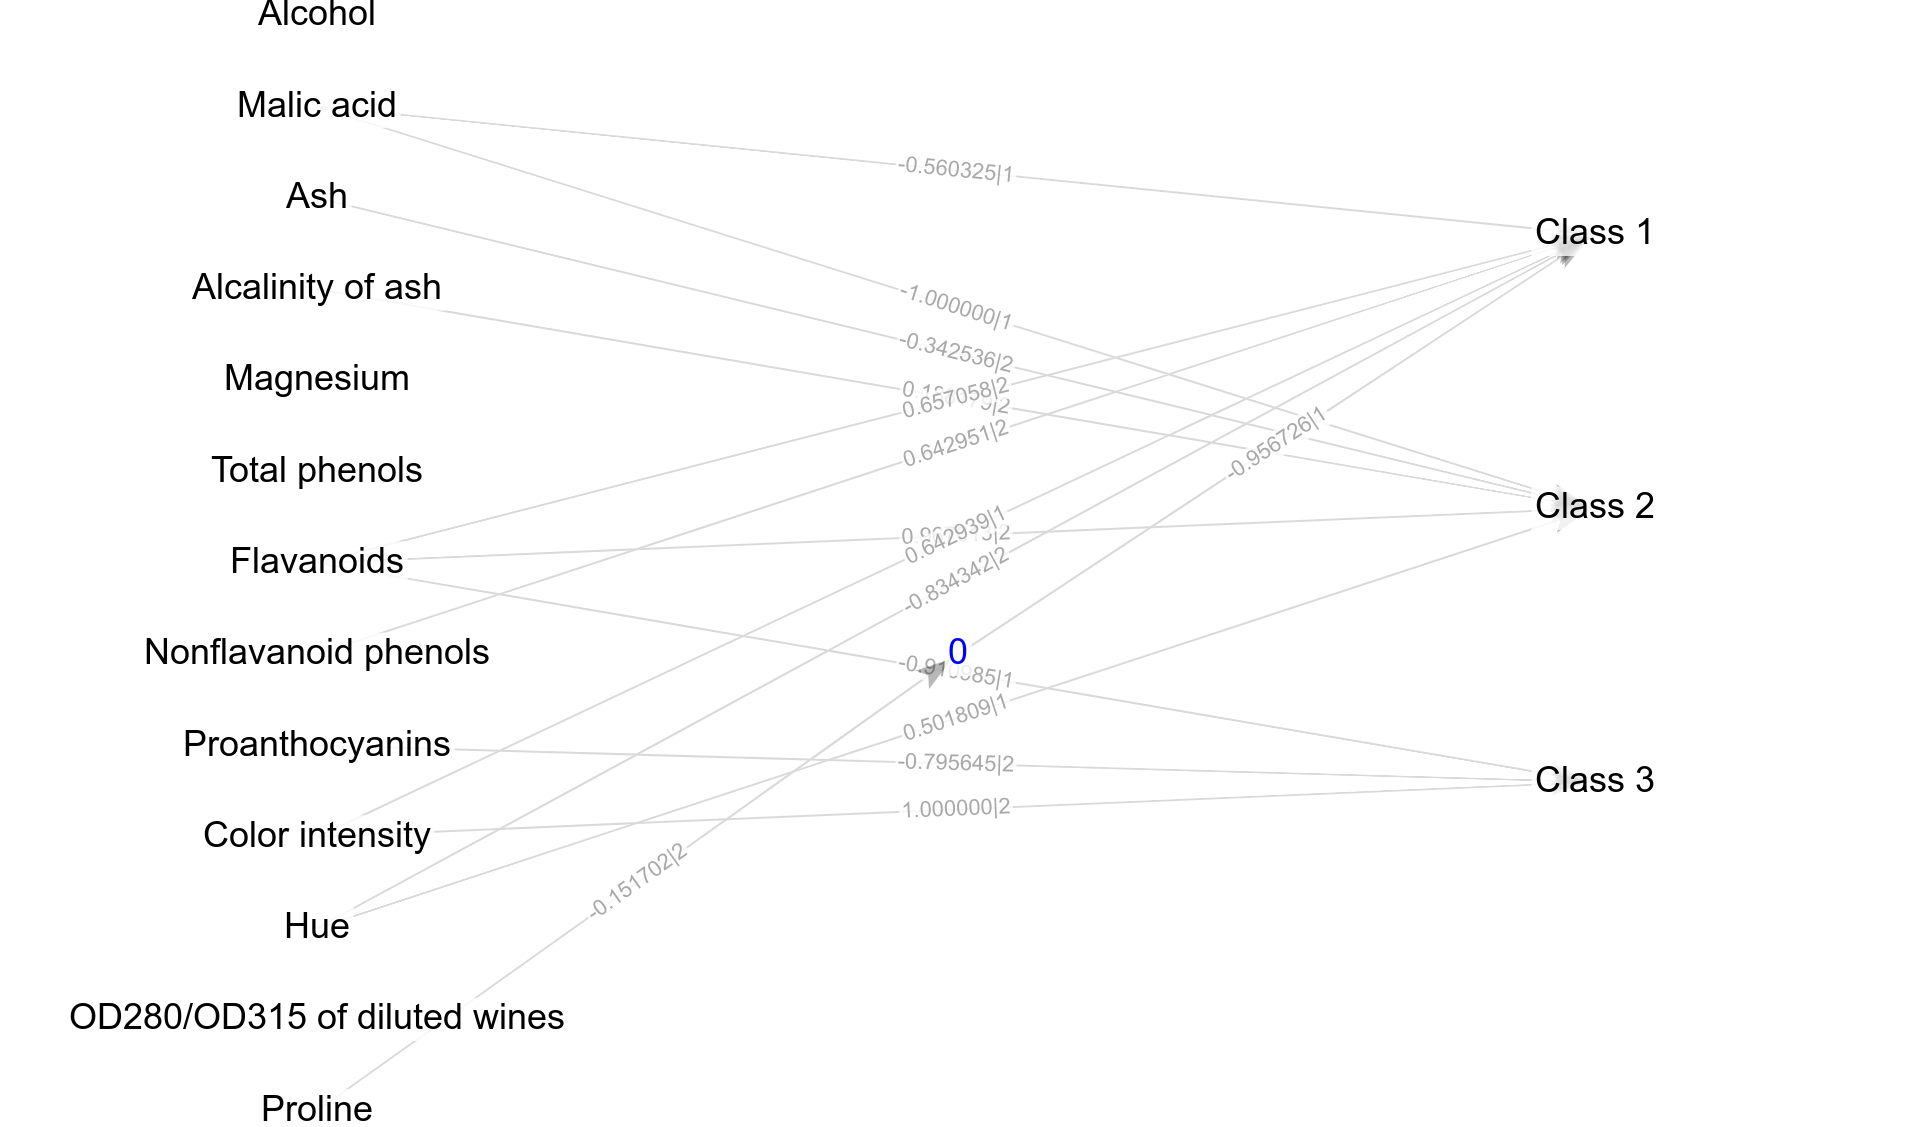
\includegraphics[width=13cm]{wine/1/mcc_g}
    \end{center}
    \caption{Vizualizacija agenta z največjim MCC prvega nabora. Vsebuje 2 globoki vozlišči in 25 povezav.}
    \label{fig:wine_mcc_1_g}
\end{figure}

\subsubsection{Drugi nabor}
%%"/home/jure/CLionProjects/Neuroevolution/datasets/iris/iris.data" 250 20 50 3 true 0.1 100 true -0.001 -0.001 350 ACC
\begin{table}[H]
    \caption{Rezultat drugega nabora parametrov.}
    \begin{center}
        \begin{tabular}{|| c | c c || c c ||}
            \hline
            \multirow{2}{*}{št. zagona} & \multicolumn{2}{c||}{točnost najboljšega agenta} & \multicolumn{2}{c||}{MCC najboljšega agenta} \\ \cline{2-5}
            & učna    & testna           & učna  & testna         \\
            \hline
            1        & 0.912\% & 0.792\%          & 0.814 & 0.860          \\
            \hline
            2        & 0.912\% & 0.830\%          & 0.879 & \textbf{0.915} \\
            \hline
            3        & 0.960\% & \textbf{0.925\%} & 0.939 & 0.888          \\
            \hline
            4        & 0.960\% & 0.887\%          & 0.879 & 0.885          \\
            \hline
            5        & 0.920\% & 0.868\%          & 0.893 & 0.786          \\
            \hline
            $\sigma$ & 0.022   & 0.077            & 0.040 & 0.044          \\
            \hline
        \end{tabular}
    \end{center}
    \label{tab:wine_result_2}
\end{table}

\begin{table}[H]
    \centering
    \caption{Matrika zmot najbolj točnega agenta drugega nabora.}
    \begin{tabular}{||rcccc||}
        \hline
        razred  & Class 1 & Class 2 & Class 3 & vsota \\ \hline
        Class 1 & 16      & 2       & 0       & 18    \\ \hline
        Class 2 & 0       & 19      & 2       & 21    \\ \hline
        Class 3 & 0       & 0       & 14      & 14    \\ \hline
        vsota   & 16      & 21      & 16      & 53    \\ \hline
    \end{tabular}
    \label{tab:wine_acc_2}
\end{table}

\begin{table}[H]
    \centering
    \caption{Matrika zmot agenta z največjim MCC drugega nabora.}
    \begin{tabular}{||rcccc||}
        \hline
        razred  & Class 1 & Class 2 & Class 3 & vsota \\ \hline
        Class 1 & 18      & 0       & 0       & 18    \\ \hline
        Class 2 & 0       & 19      & 2       & 21    \\ \hline
        Class 3 & 0       & 1       & 13      & 14    \\ \hline
        vsota   & 18      & 20      & 15      & 53    \\ \hline
    \end{tabular}
    \label{tab:wine_mcc_2}
\end{table}

\begin{figure}[H]
    \begin{center}
        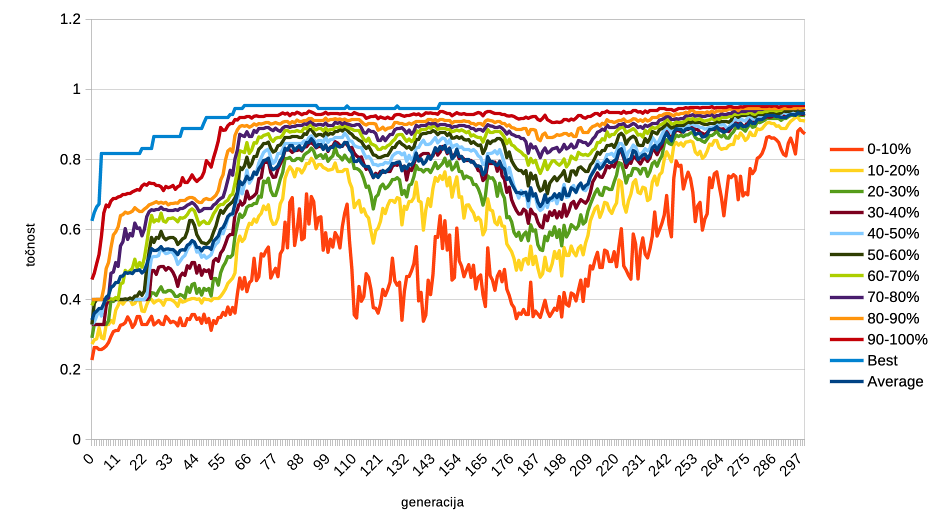
\includegraphics[width=13cm]{wine/2/acc}
    \end{center}
    \caption{Graf točnosti populacije najboljšega agenta drugega nabora skozi generacije.}
    \label{fig:wine_acc_2}
\end{figure}

\begin{figure}[H]
    \begin{center}
        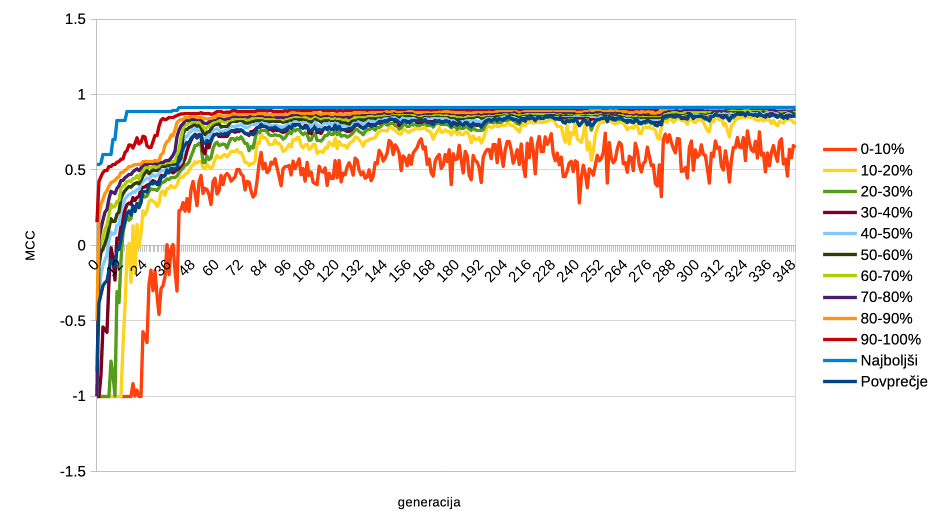
\includegraphics[width=13cm]{wine/2/mcc}
    \end{center}
    \caption{Graf MCC populacije najboljšega agenta drugega nabora skozi generacije.}
    \label{fig:wine_mcc_2}
\end{figure}

\begin{figure}[H]
    \begin{center}
        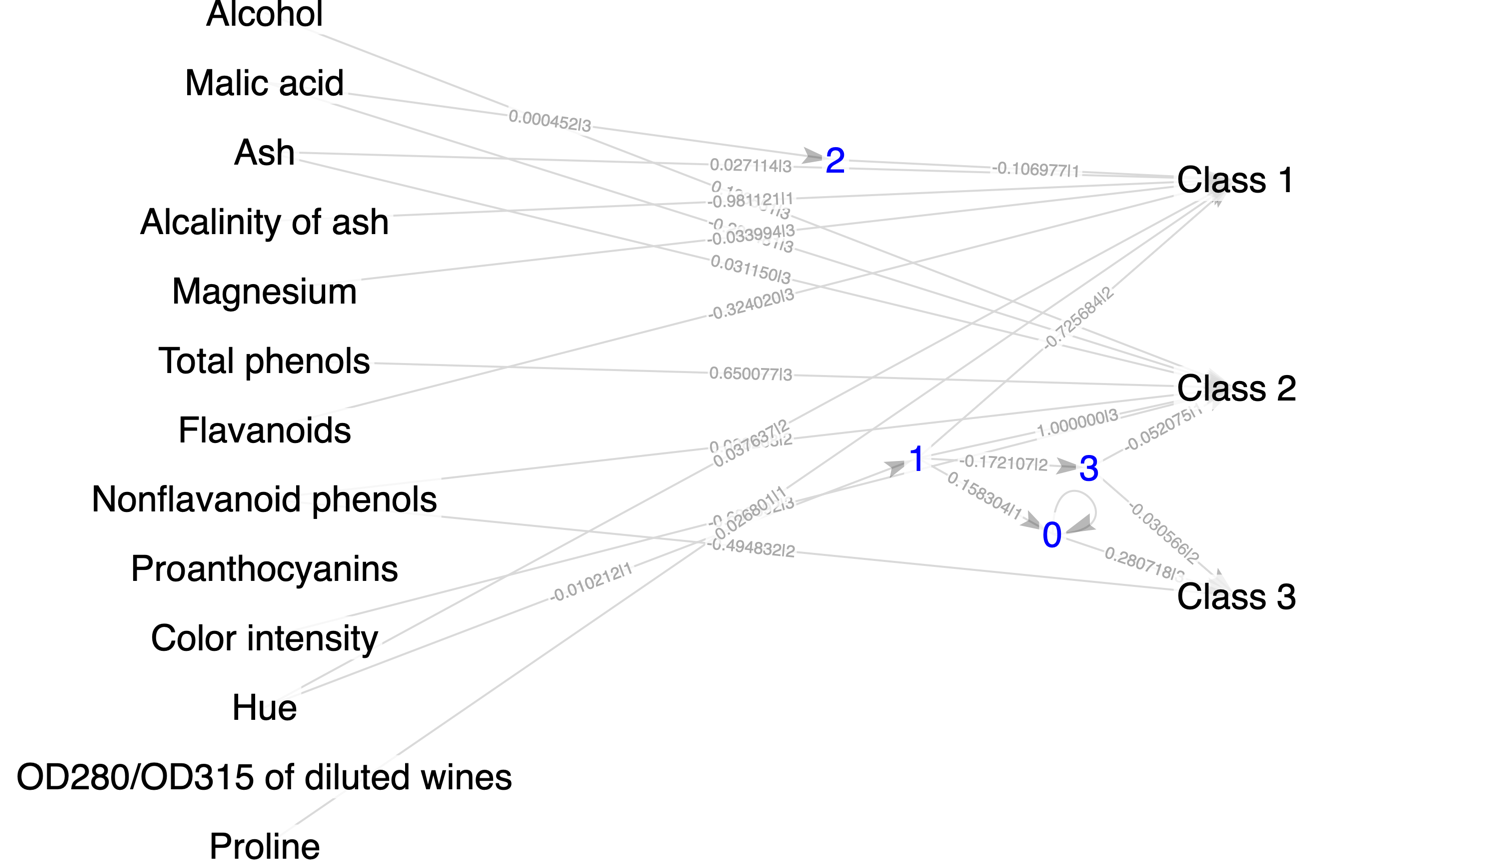
\includegraphics[width=13cm]{wine/2/acc_g}
    \end{center}
    \caption{Vizualizacija najbolj točnega agenta drugega nabora. Vsebuje 4 globoka vozlišča in 24 povezav.}
    \label{fig:wine_acc_2_g}
\end{figure}

\begin{figure}[H]
    \begin{center}
        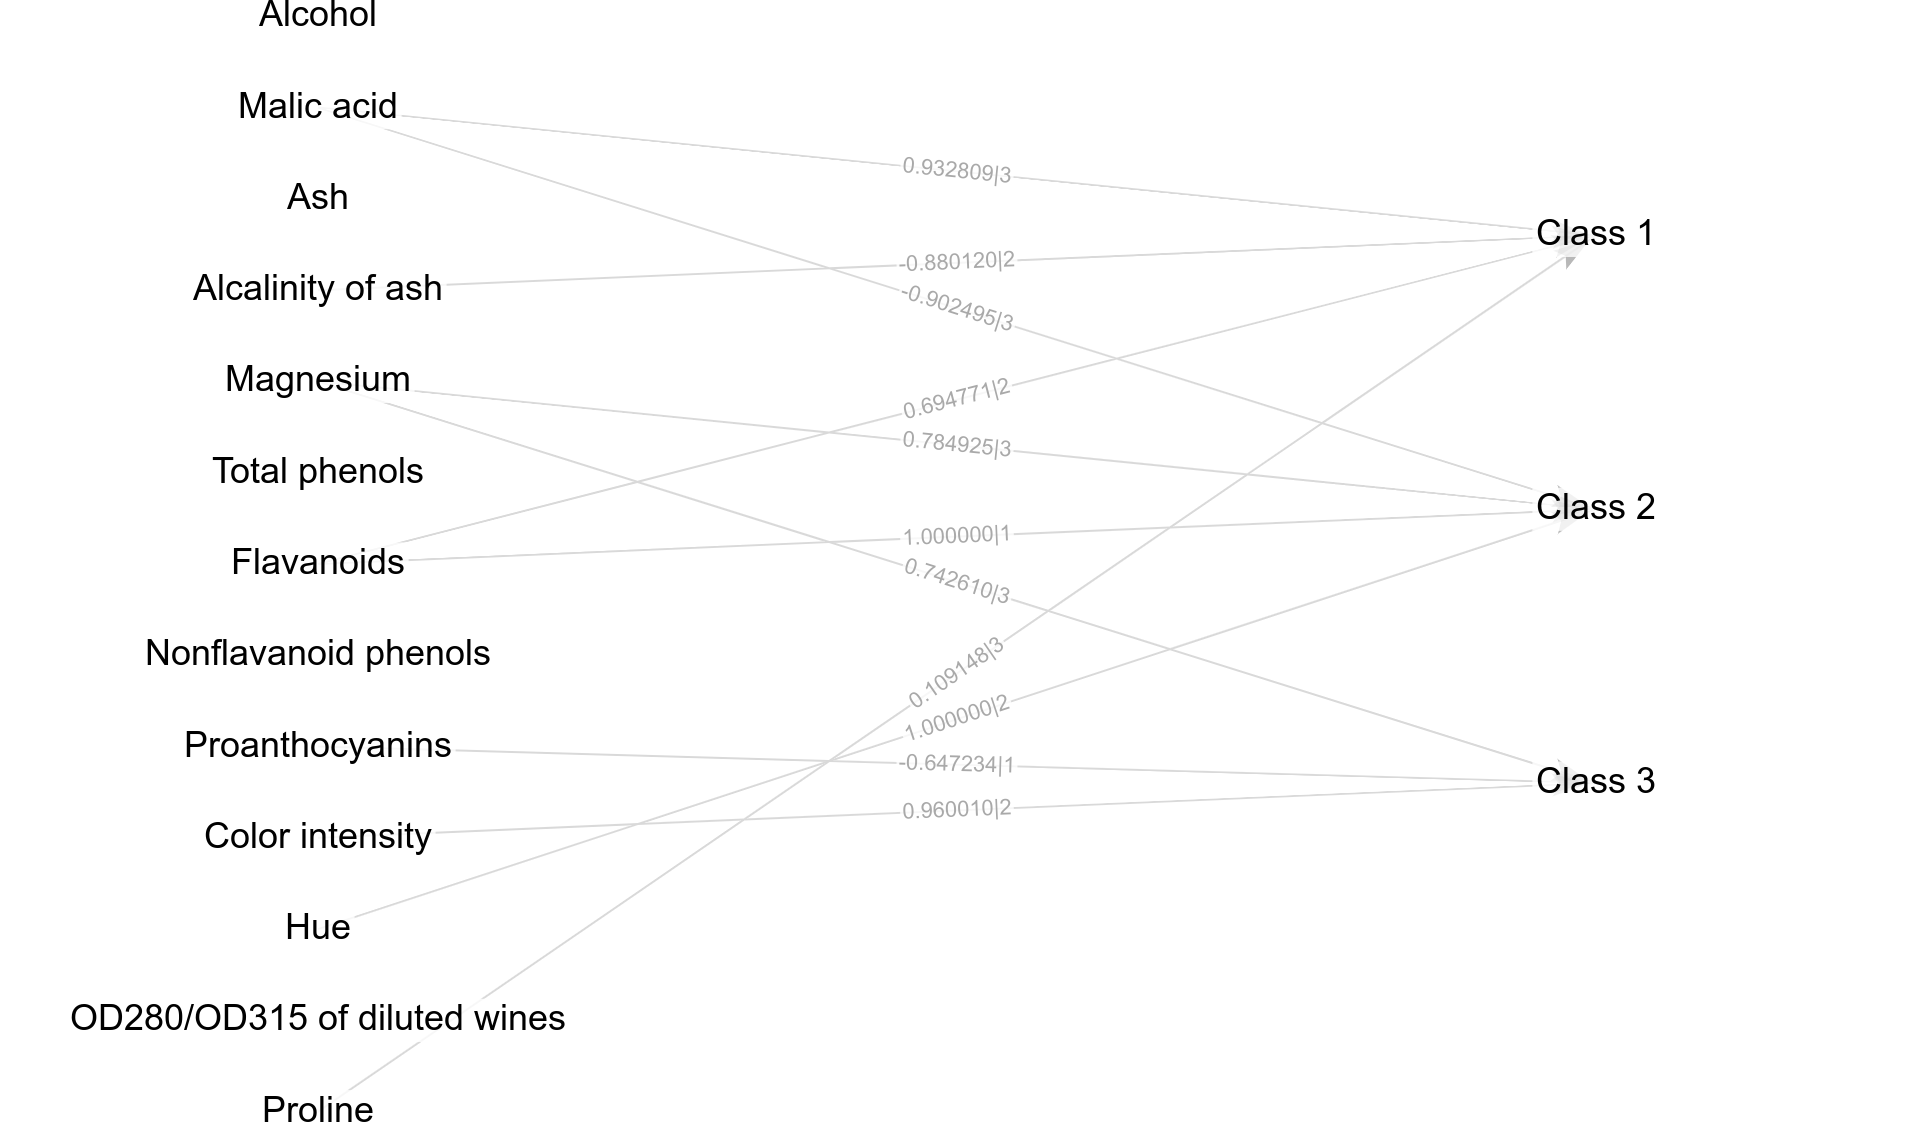
\includegraphics[width=13cm]{wine/2/mcc_g}
    \end{center}
    \caption{Vizualizacija agenta z največjim MCC drugega nabora. Vsebuje 10 globokih vozlišč in 47 povezav.}
    \label{fig:wine_mcc_2_g}
\end{figure}

\subsubsection{Tretji nabor}
%%"/home/jure/CLionProjects/Neuroevolution/datasets/iris/iris.data" 350 25 75 4 true 0.1 175 true -0.001 -0.001 450 ACC
\begin{table}[H]
    \caption{Rezultat tretjega nabora parametrov.}
    \begin{center}
        \begin{tabular}{|| c | c c || c c ||}
            \hline
            \multirow{2}{*}{št. zagona} & \multicolumn{2}{c||}{točnost najboljšega agenta} & \multicolumn{2}{c||}{MCC najboljšega agenta} \\ \cline{2-5}
            & učna    & testna           & učna  & testna         \\
            \hline
            1        & 0.896\% & 0.925\%          & 0.861 & 0.843          \\
            \hline
            2        & 0.912\% & 0.755\%          & 0.871 & 0.772          \\
            \hline
            3        & 0.928\% & 0.868\%          & 0.903 & 0.887          \\
            \hline
            4        & 0.896\% & 0.906\%          & 0.976 & 0.858          \\
            \hline
            5        & 0.960\% & \textbf{0.943\%} & 0.952 & \textbf{0.972} \\
            \hline
            $\sigma$ & 0.024   & 0.067            & 0.045 & 0.065          \\
            \hline
        \end{tabular}
    \end{center}
    \label{tab:wine_result_3}
\end{table}

\begin{table}[H]
    \centering
    \caption{Matrika zmot najbolj točnega agenta tretjega nabora (zagon 3).}
    \begin{tabular}{||rcccc||}
        \hline
        razred  & Class 1 & Class 2 & Class 3 & vsota \\ \hline
        Class 1 & 15      & 3       & 0       & 18    \\ \hline
        Class 2 & 0       & 21      & 0       & 21    \\ \hline
        Class 3 & 0       & 0       & 14      & 14    \\ \hline
        vsota   & 15      & 24      & 14      & 53    \\ \hline
    \end{tabular}
    \label{tab:wine_acc_3}
\end{table}

\begin{table}[H]
    \centering
    \caption{Matrika zmot agenta z največjim MCC tretjega nabora.}
    \begin{tabular}{||rcccc||}
        \hline
        razred  & Class 1 & Class 2 & Class 3 & vsota \\ \hline
        Class 1 & 17      & 1       & 0       & 18    \\ \hline
        Class 2 & 0       & 21      & 0       & 21    \\ \hline
        Class 3 & 0       & 0       & 14      & 14    \\ \hline
        vsota   & 17      & 22      & 14      & 53    \\ \hline
    \end{tabular}
    \label{tab:wine_mcc_3}
\end{table}

\begin{figure}[H]
    \begin{center}
        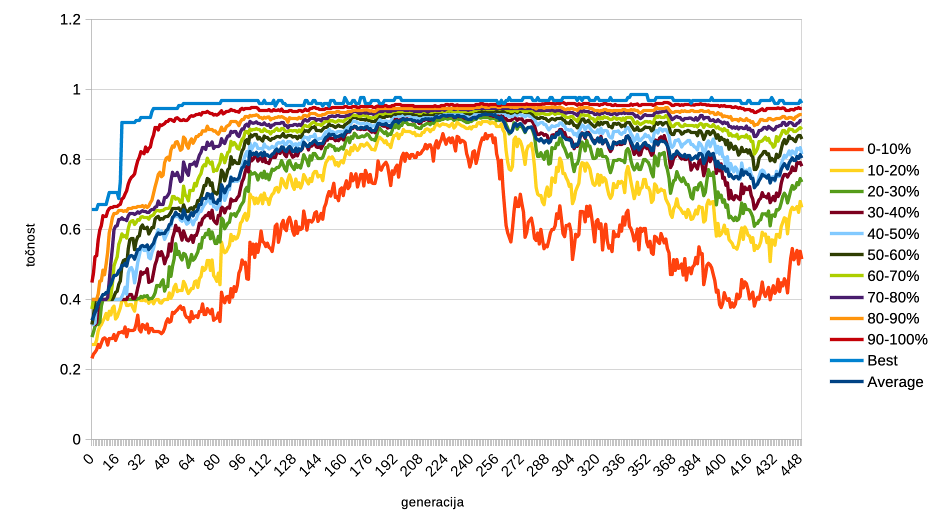
\includegraphics[width=13cm]{wine/3/acc}
    \end{center}
    \caption{Graf točnosti populacije najboljšega agenta tretjega nabora skozi generacije.}
    \label{fig:wine_acc_3}
\end{figure}

\begin{figure}[H]
    \begin{center}
        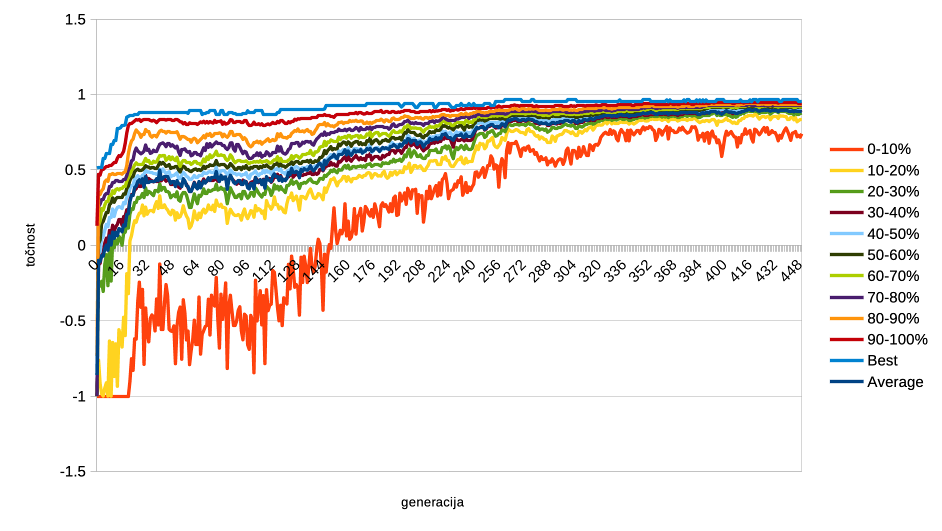
\includegraphics[width=13cm]{wine/3/mcc}
    \end{center}
    \caption{Graf MCC populacije najboljšega agenta tretjega nabora skozi generacije.}
    \label{fig:wine_mcc_3}
\end{figure}

\begin{figure}[H]
    \begin{center}
        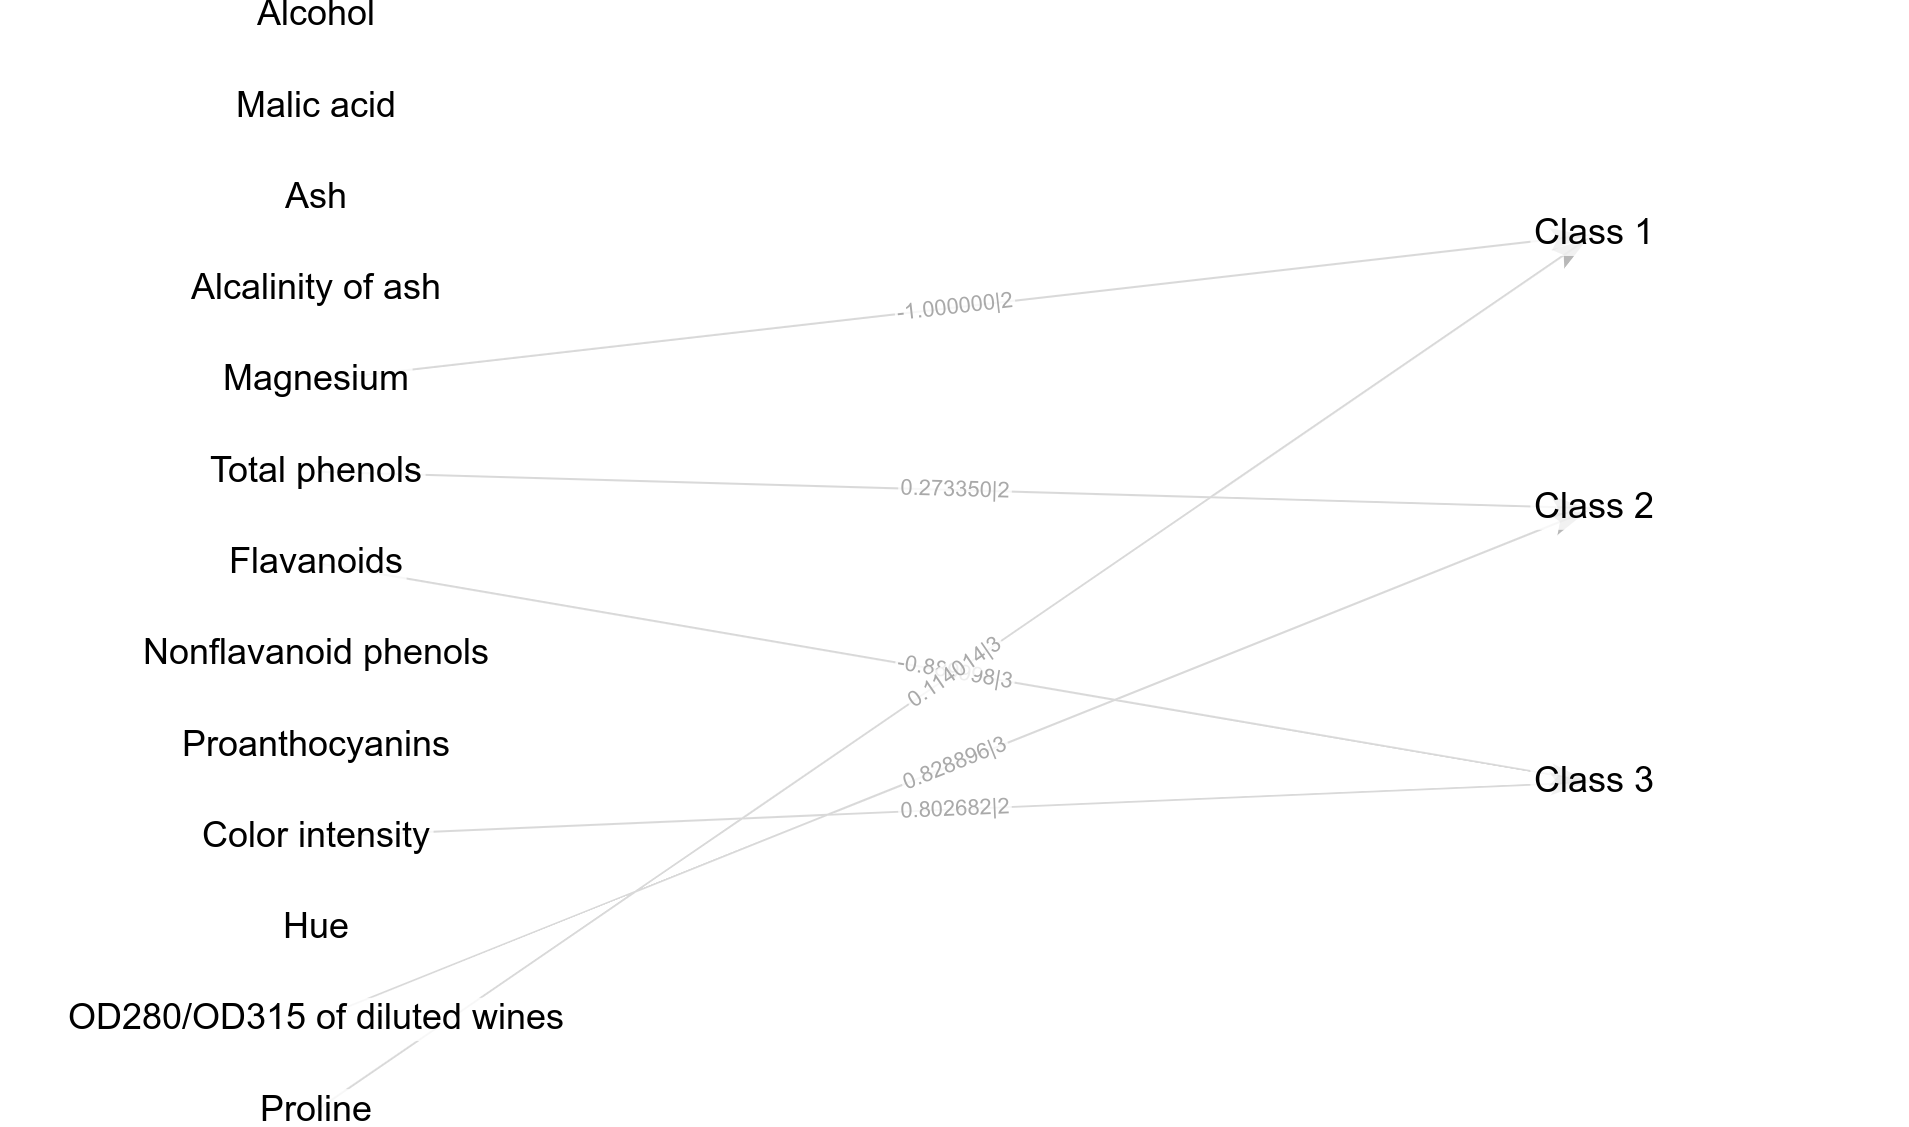
\includegraphics[width=13cm]{wine/3/acc_g}
    \end{center}
    \caption{Vizualizacija najbolj točnega agenta tretjega nabora. Vsebuje 4 globoka vozlišča in 37 povezav.}
    \label{fig:wine_acc_3_g}
\end{figure}

\begin{figure}[H]
    \begin{center}
        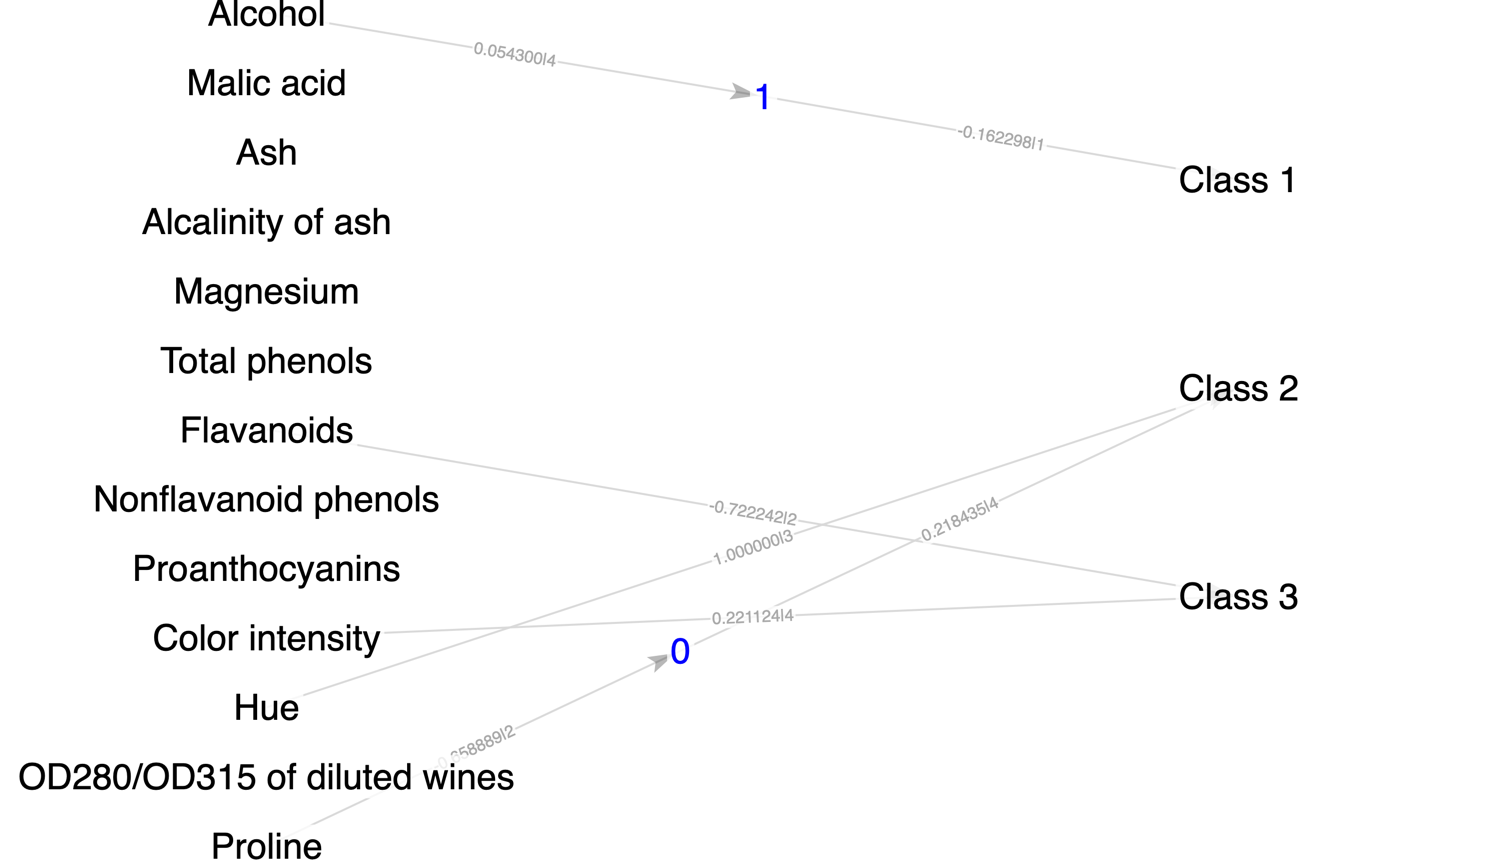
\includegraphics[width=13cm]{wine/3/mcc_g}
    \end{center}
    \caption{Vizualizacija agenta z največjim MCC tretjega nabora. Vsebuje 9 globokih vozlišč in 67 povezav.}
    \label{fig:wine_mcc_3_g}
\end{figure}

\subsection{Car Evaluation}\label{subsec:car_test}
%% arrowLength=10
%% linkWidth=3
%% input fy=50*node.pos
%% output fx=350
%% output fy=50*node.pos+50
%% MAX_FONT_SIZE=8
\begin{table}[H]
    \caption{Nabori inicializacijskih parametrov poganjanja na množici Car Evaluation.}
    \begin{center}
        \begin{tabular}{||l c c c||}
            \hline
            & 1        & 2        & 3 \\ [0.5ex]
            \hline
            velikost populacije               & 200      & 250      & 350      \\
            \hline
            največje število globokih vozlišč & 15       & 20       & 40       \\
            \hline
            največje število povezav          & 30       & 50       & 100      \\
            \hline
            največje število prečkanj         & 2        & 3        & 4        \\
            \hline
            delež mutiranih potomcev          & 10\%     & 10\%     & 10\%     \\
            \hline
            prispevek vozlišč                 & -0.00001 & -0.00001 & -0.00001 \\
            \hline
            prispevek povezav                 & -0.00001 & -0.00001 & -0.00001 \\
            \hline
            število generacij                 & 200      & 200      & 300      \\
            \hline
        \end{tabular}
    \end{center}
    \label{tab:param_car}
\end{table}

\subsubsection{Prvi nabor}
%%"/home/jure/CLionProjects/Neuroevolution/datasets/car/car.data" 200 15 30 2 true 0.1 100 true -0.00001 -0.00001 300 ACC
\begin{table}[H]
    \caption{Rezultat prvega nabora parametrov.}
    \begin{center}
        \begin{tabular}{|| c | c c || c c ||}
            \hline
            \multirow{2}{*}{št. zagona} & \multicolumn{2}{c||}{točnost najboljšega agenta} & \multicolumn{2}{c||}{MCC najboljšega agenta} \\ \cline{2-5}
            & učna    & testna           & učna  & testna         \\
            \hline
            1        & 0.729\% & \textbf{0.724\%} & 0.439 & 0.404          \\
            \hline
            2        & 0.721\% & 0.718\%          & 0.464 & 0.441          \\
            \hline
            3        & 0.732\% & 0.716\%          & 0.506 & 0.456          \\
            \hline
            4        & 0.715\% & 0.720\%          & 0.495 & 0.485          \\
            \hline
            5        & 0.719\% & 0.705\%          & 0.493 & \textbf{0.488} \\
            \hline
            $\sigma$ & 0.020   & 0.006            & 0.025 & 0.031          \\
            \hline
        \end{tabular}
    \end{center}
    \label{tab:car_result_1}
\end{table}

\begin{table}[H]
    \centering
    \caption{Matrika zmot najbolj točnega agenta prvega nabora. Agent lahko napove samo razreda \enquote{nesprejemljivo} in \enquote{sprejemljivo}.}
    \begin{tabular}{||rccccc||}
        \hline
        razred       & unacceptable & acceptable & good & very good & vsota \\ \hline
        unacceptable & 357          & 6          & 0    & 0         & 363   \\ \hline
        acceptable   & 97           & 18         & 0    & 0         & 115   \\ \hline
        good         & 13           & 8          & 0    & 0         & 21    \\ \hline
        very good    & 9            & 10         & 0    & 0         & 19    \\ \hline
        vsota        & 476          & 42         & 0    & 0         & 518   \\ \hline
    \end{tabular}
    \label{tab:car_acc_1}
\end{table}

\begin{table}[H]
    \centering
    \caption{Matrika zmot agenta z največjim MCC prvega nabora. Agent lahko napove samo razreda \enquote{nesprejemljivo} in \enquote{sprejemljivo}.}
    \begin{tabular}{||rccccc||}
        \hline
        razred       & unacceptable & acceptable & good & very good & vsota \\ \hline
        unacceptable & 260          & 103        & 0    & 0         & 363   \\ \hline
        acceptable   & 10           & 105        & 0    & 0         & 115   \\ \hline
        good         & 0            & 21         & 0    & 0         & 21    \\ \hline
        very good    & 0            & 19         & 0    & 0         & 19    \\ \hline
        vsota        & 270          & 248        & 0    & 0         & 518   \\ \hline
    \end{tabular}
    \label{tab:car_mcc_1}
\end{table}

\begin{figure}[H]
    \begin{center}
        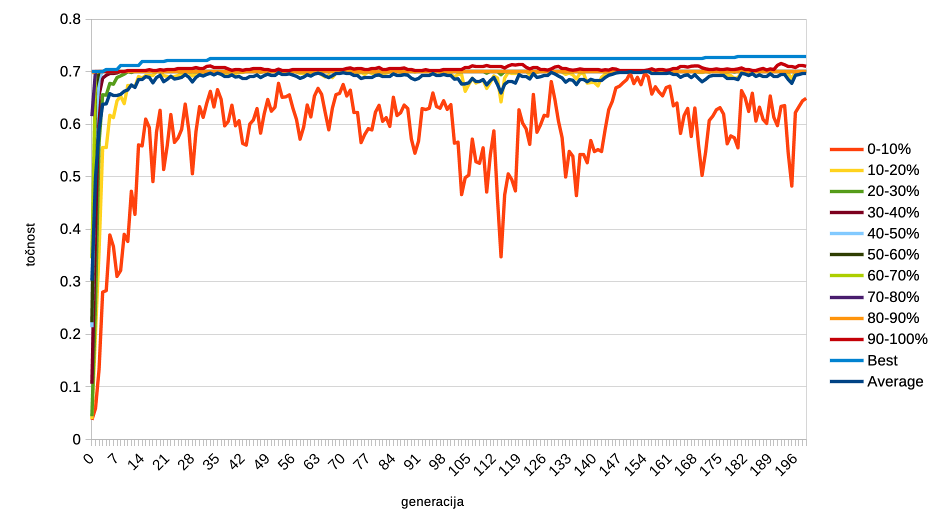
\includegraphics[width=13cm]{car/1/acc}
    \end{center}
    \caption{Graf točnosti populacije najboljšega agenta prvega nabora skozi generacije.}
    \label{fig:car_acc_1}
\end{figure}

\begin{figure}[H]
    \begin{center}
        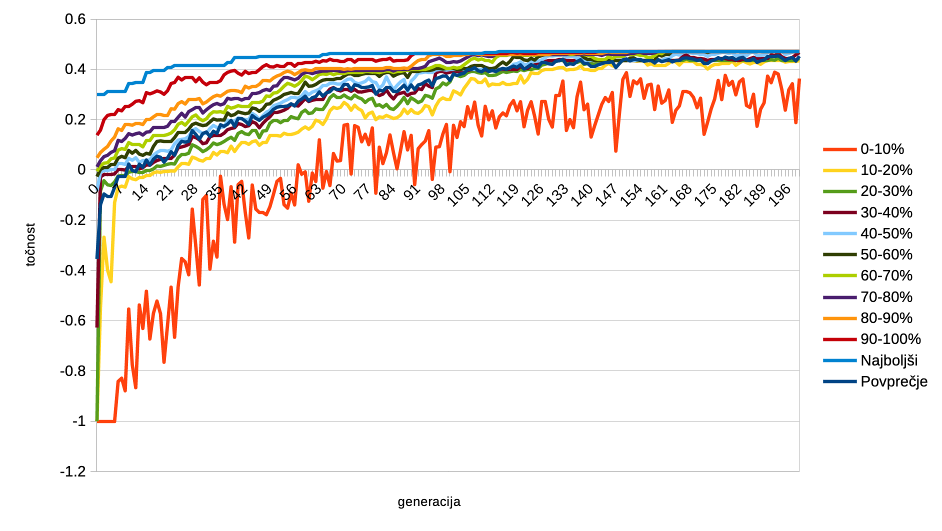
\includegraphics[width=13cm]{car/1/mcc}
    \end{center}
    \caption{Graf MCC populacije najboljšega agenta prvega nabora skozi generacije.}
    \label{fig:car_mcc_1}
\end{figure}

\begin{figure}[H]
    \begin{center}
        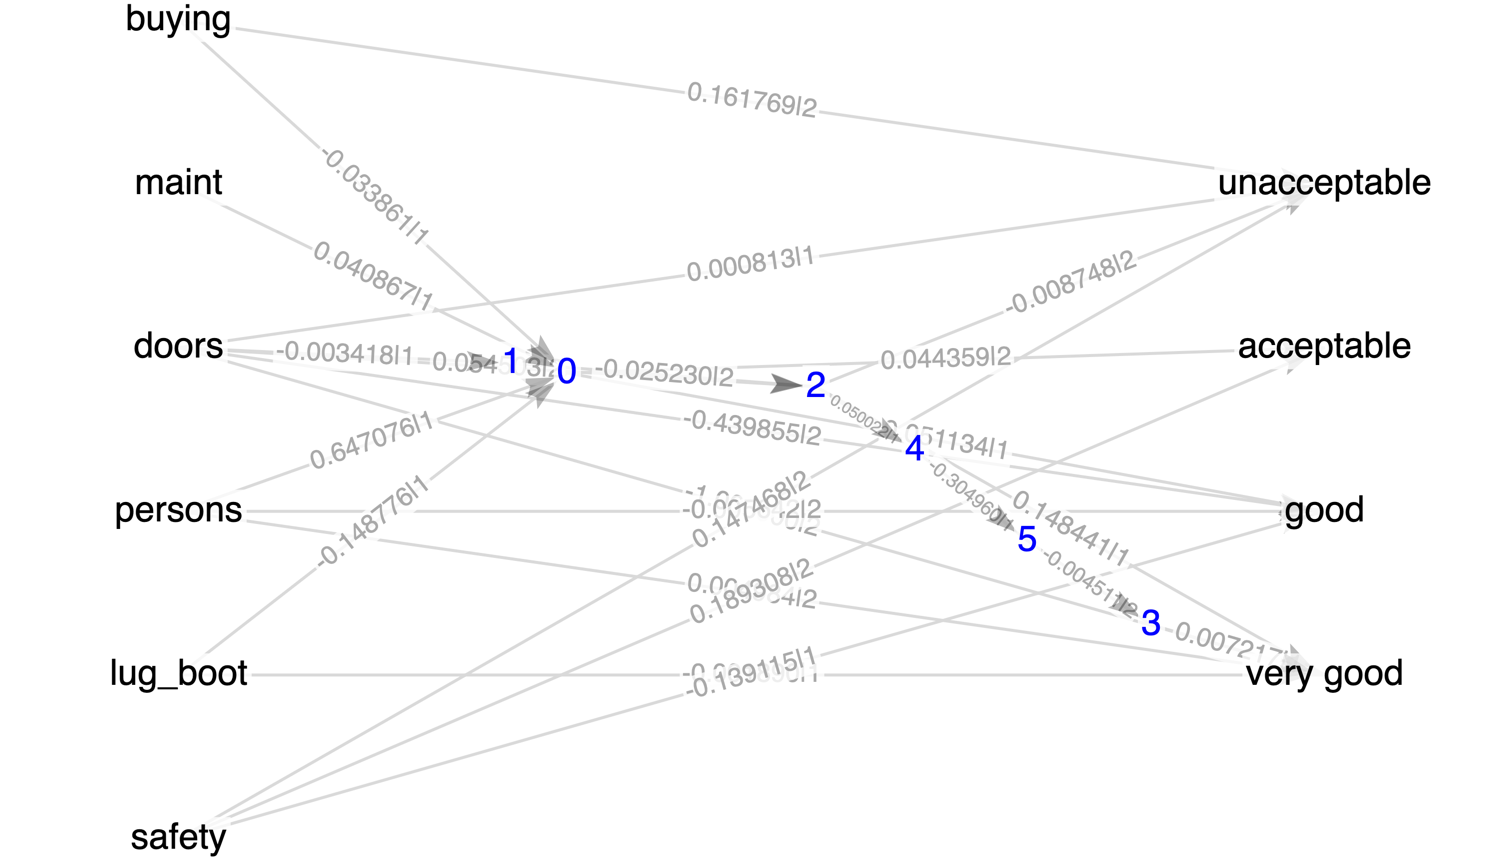
\includegraphics[width=13cm]{car/1/acc_g}
    \end{center}
    \caption{Vizualizacija najbolj točnega agenta prvega nabora. Vsebuje 6 globokih vozlišč in 25 povezav.}
    \label{fig:car_acc_1_g}
\end{figure}

\begin{figure}[H]
    \begin{center}
        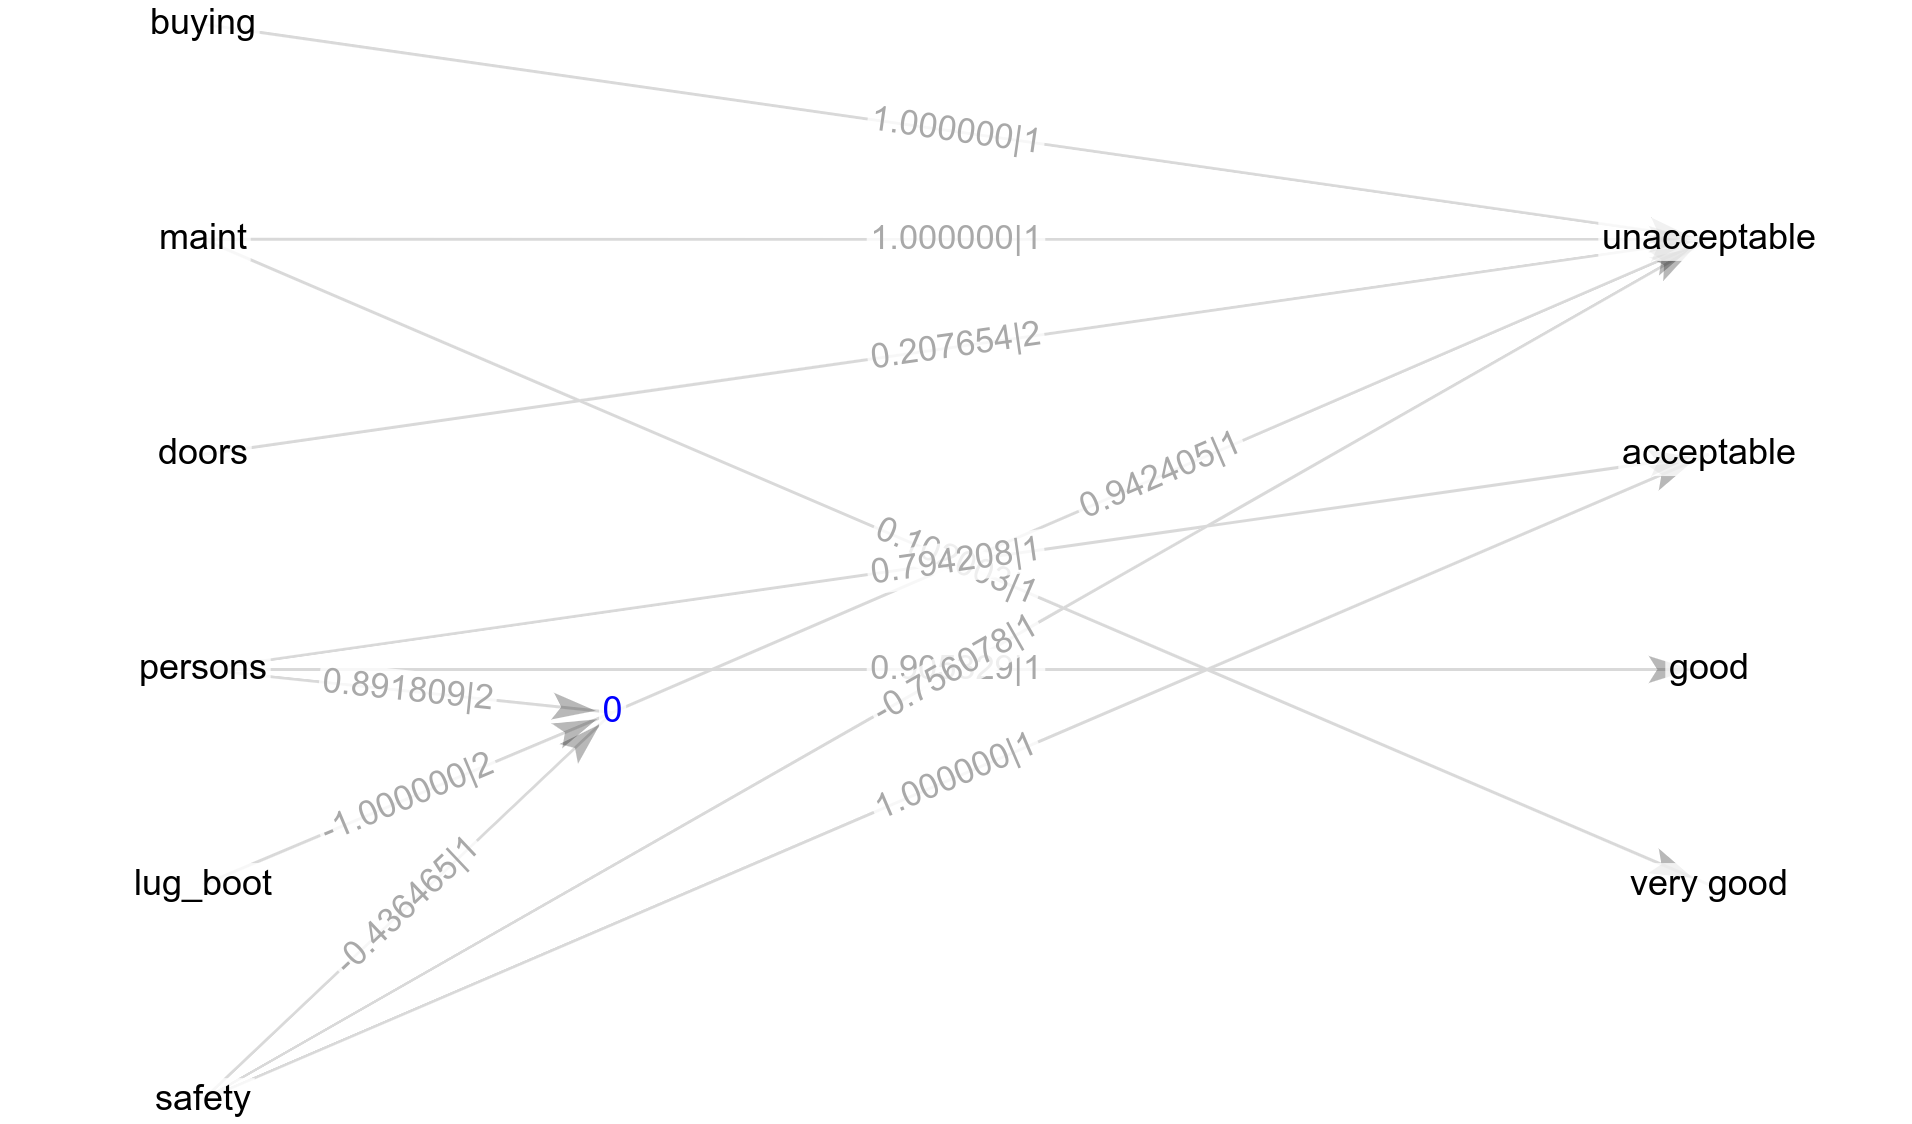
\includegraphics[width=13cm]{car/1/mcc_g}
    \end{center}
    \caption{Vizualizacija agenta z največjim MCC prvega nabora. Vsebuje 5 globokih vozlišč in 23 povezav.}
    \label{fig:car_mcc_1_g}
\end{figure}

\subsubsection{Drugi nabor}
%% 250 20 50 3 true 0.1 125 true -0.00001 -0.00001 200 ACC
\begin{table}[H]
    \caption{Rezultat drugega nabora parametrov.}
    \begin{center}
        \begin{tabular}{|| c | c c || c c ||}
            \hline
            \multirow{2}{*}{št. zagona} & \multicolumn{2}{c||}{točnost najboljšega agenta} & \multicolumn{2}{c||}{MCC najboljšega agenta} \\ \cline{2-5}
            & učna    & testna           & učna  & testna         \\
            \hline
            1        & 0.729\% & 0.716\%          & 0.505 & 0.471          \\
            \hline
            2        & 0.716\% & 0.718\%          & 0.486 & 0.507          \\
            \hline
            3        & 0.707\% & 0.701\%          & 0.475 & \textbf{0.530} \\
            \hline
            4        & 0.719\% & \textbf{0.724\%} & 0.482 & 0.513          \\
            \hline
            5        & 0.713\% & 0.695\%          & 0.501 & 0.479          \\
            \hline
            $\sigma$ & 0.007   & 0.011            & 0.011 & 0.022          \\
            \hline
        \end{tabular}
    \end{center}
    \label{tab:car_result_2}
\end{table}

\begin{table}[H]
    \centering
    \caption{Matrika zmot najbolj točnega agenta drugega nabora. Agent lahko napove samo razreda \enquote{nesprejemljivo} in \enquote{zelo dobro}.}
    \begin{tabular}{||rccccc||}
        \hline
        razred       & unacceptable & acceptable & good & very good & vsota \\ \hline
        unacceptable & 361          & 0          & 0    & 2         & 363   \\ \hline
        acceptable   & 102          & 0          & 0    & 13        & 115   \\ \hline
        good         & 15           & 0          & 0    & 6         & 21    \\ \hline
        very good    & 5            & 0          & 0    & 14        & 19    \\ \hline
        vsota        & 473          & 0          & 0    & 35        & 518   \\ \hline
    \end{tabular}
    \label{tab:car_acc_2}
\end{table}

\begin{table}[H]
    \centering
    \caption{Matrika zmot agenta z največjim MCC drugega nabora. Agent lahko napove samo razreda \enquote{nesprejemljivo} in \enquote{sprejemljivo}.}
    \begin{tabular}{||rccccc||}
        \hline
        razred       & unacceptable & acceptable & good & very good & vsota \\ \hline
        unacceptable & 276          & 87         & 0    & 0         & 363   \\ \hline
        acceptable   & 9            & 106        & 0    & 0         & 115   \\ \hline
        good         & 0            & 21         & 0    & 0         & 21    \\ \hline
        very good    & 0            & 19         & 0    & 0         & 19    \\ \hline
        vsota        & 285          & 233        & 0    & 0         & 518   \\ \hline
    \end{tabular}
    \label{tab:car_mcc_2}
\end{table}

\begin{figure}[H]
    \begin{center}
        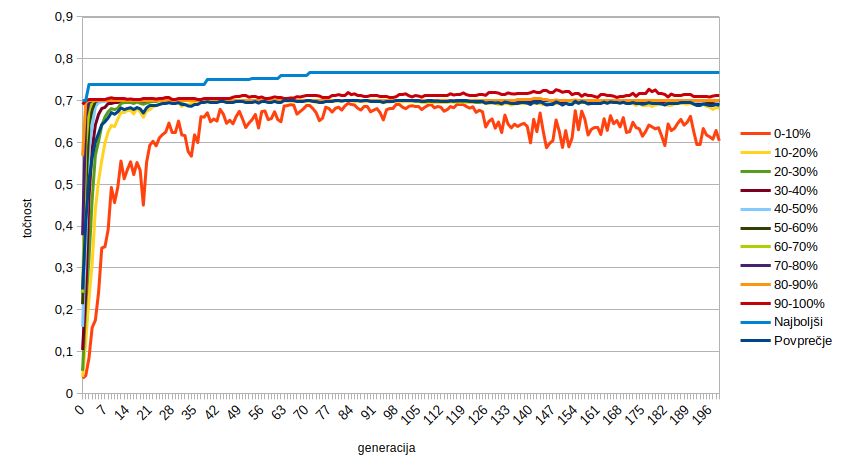
\includegraphics[width=13cm]{car/2/acc}
    \end{center}
    \caption{Graf točnosti populacije najboljšega agenta drugega nabora skozi generacije.}
    \label{fig:car_acc_2}
\end{figure}

\begin{figure}[H]
    \begin{center}
        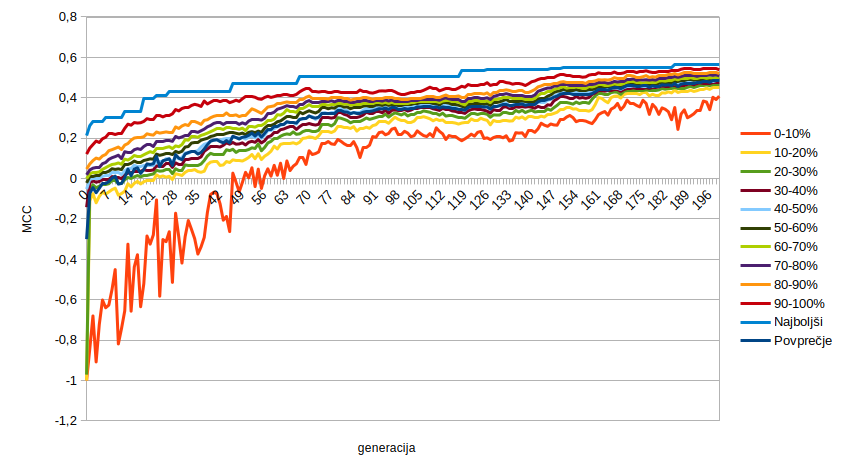
\includegraphics[width=13cm]{car/2/mcc}
    \end{center}
    \caption{Graf MCC populacije najboljšega agenta drugega nabora skozi generacije.}
    \label{fig:car_mcc_2}
\end{figure}

\begin{figure}[H]
    \begin{center}
        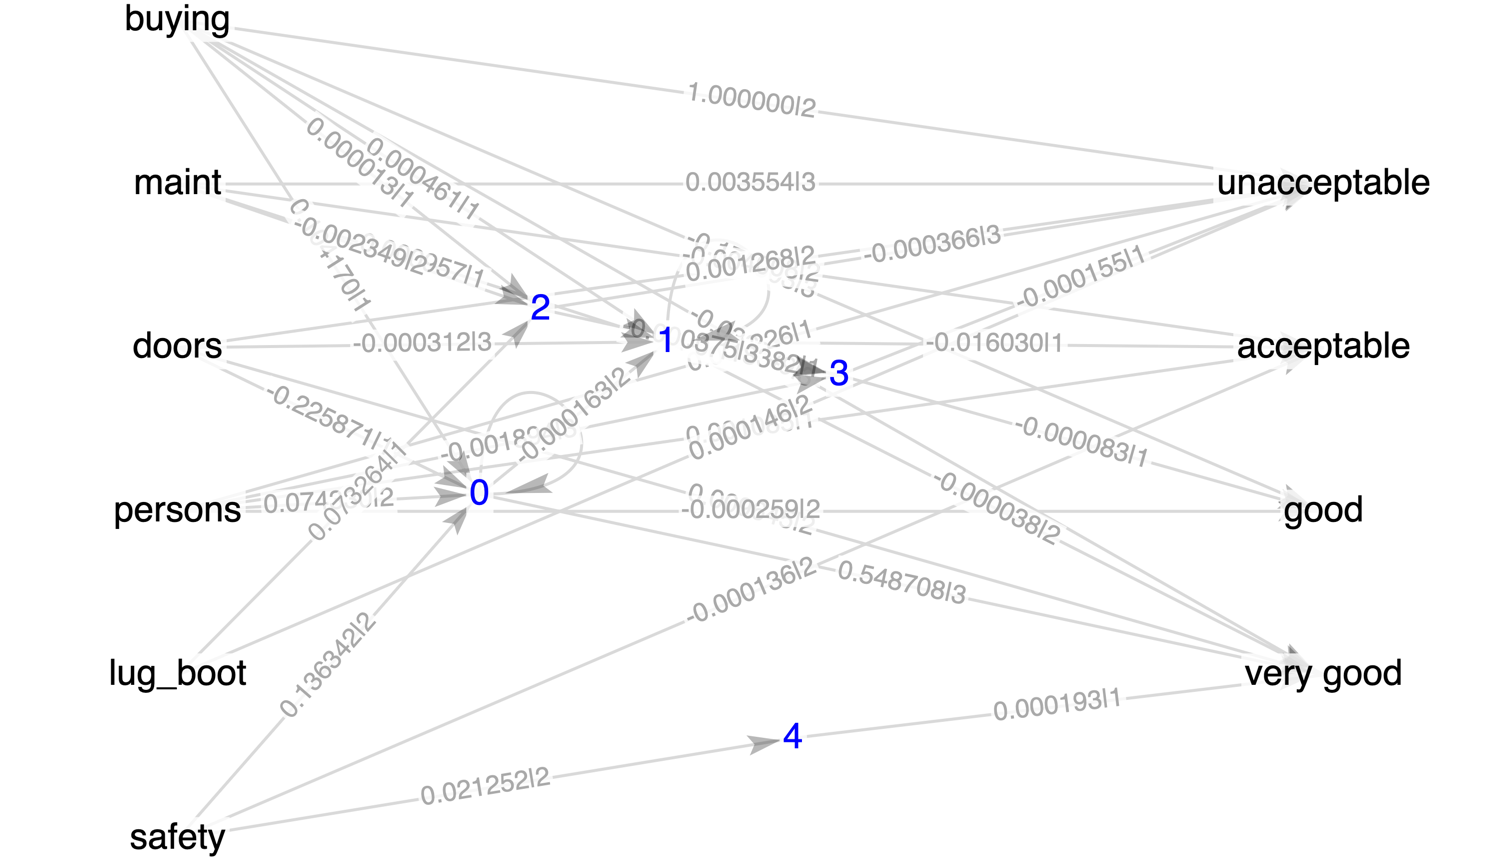
\includegraphics[width=13cm]{car/2/acc_g}
    \end{center}
    \caption{Vizualizacija najbolj točnega agenta drugega nabora. Vsebuje 5 globokih vozlišč in 36 povezav.}
    \label{fig:car_acc_2_g}
\end{figure}

\begin{figure}[H]
    \begin{center}
        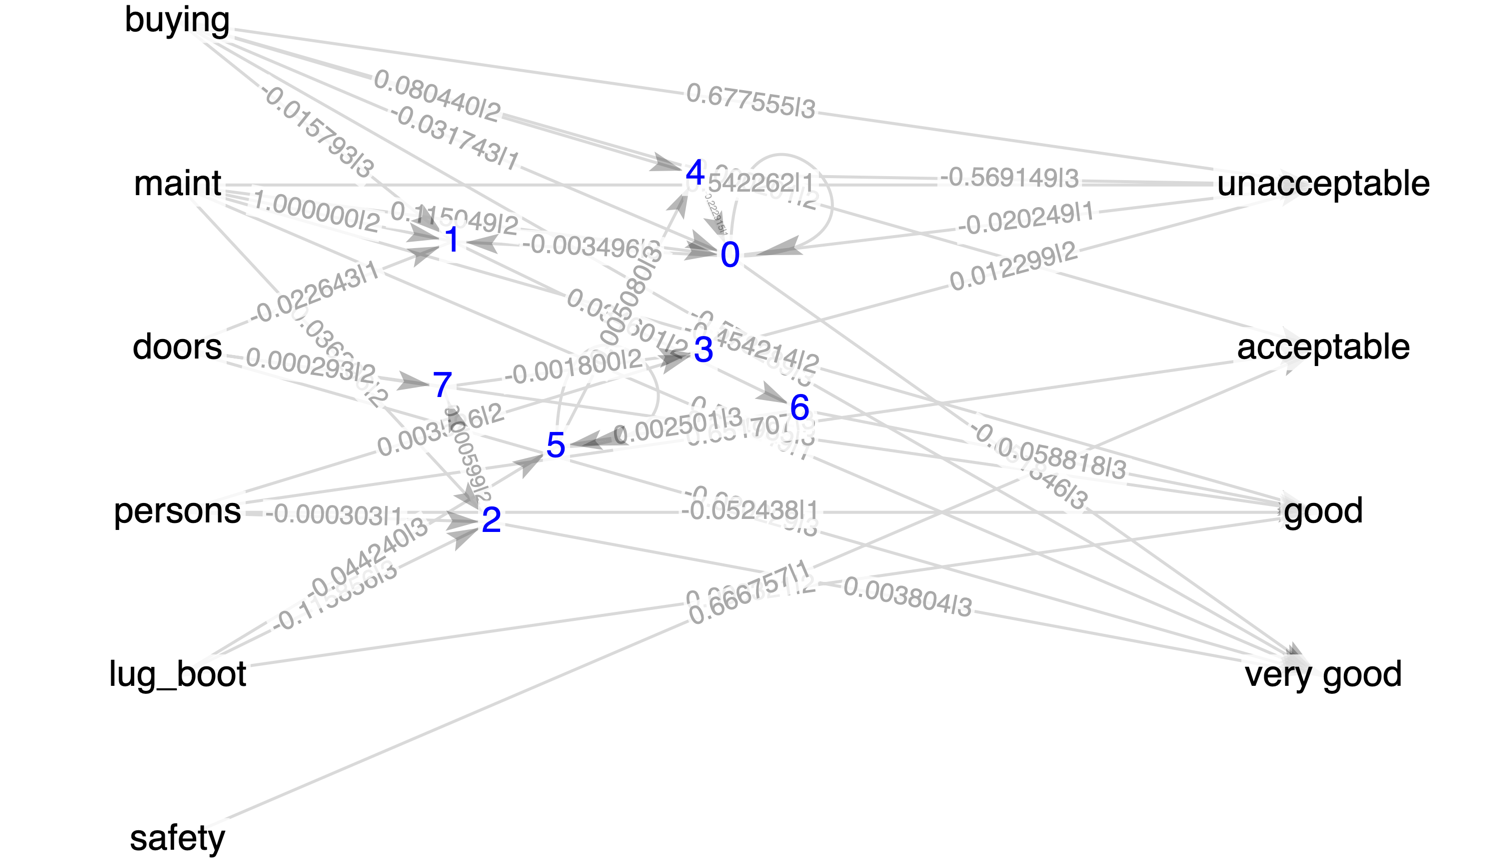
\includegraphics[width=13cm]{car/2/mcc_g}
    \end{center}
    \caption{Vizualizacija agenta z največjim MCC drugega nabora. Vsebuje 8 globokih vozlišč in 39 povezav.}
    \label{fig:car_mcc_2_g}
\end{figure}

\subsubsection{Tretji nabor}
%% 350 40 100 4 true 0.1 175 true -0.00001 -0.00001 300 ACC
\begin{table}[H]
    \caption{Rezultat tretjega nabora parametrov.}
    \begin{center}
        \begin{tabular}{|| c | c c || c c ||}
            \hline
            \multirow{2}{*}{št. zagona} & \multicolumn{2}{c||}{točnost najboljšega agenta} & \multicolumn{2}{c||}{MCC najboljšega agenta} \\ \cline{2-5}
            & učna    & testna           & učna  & testna         \\
            \hline
            1        & 0.716\% & 0.708\%          & 0.471 & 0.480          \\
            \hline
            2        & 0.719\% & 0.705\%          & 0.502 & 0.473          \\
            \hline
            3        & 0.729\% & 0.728\%          & 0.482 & \textbf{0.486} \\
            \hline
            4        & 0.740\% & 0.716\%          & 0.512 & 0.443          \\
            \hline
            5        & 0.737\% & \textbf{0.734\%} & 0.501 & 0.479          \\
            \hline
            $\sigma$ & 0.009   & 0.011            & 0.015 & 0.015          \\
            \hline
        \end{tabular}
    \end{center}
    \label{tab:car_result_3}
\end{table}

\begin{table}[H]
    \centering
    \caption{Matrika zmot najbolj točnega agenta tretjega nabora. Agent lahko napove samo razreda \enquote{nesprejemljivo} in \enquote{sprejemljivo}.}
    \begin{tabular}{||rccccc||}
        \hline
        razred       & unacceptable & acceptable & good & very good & vsota \\ \hline
        unacceptable & 306          & 57         & 0    & 0         & 363   \\ \hline
        acceptable   & 41           & 74         & 0    & 0         & 115   \\ \hline
        good         & 0            & 21         & 0    & 0         & 21    \\ \hline
        very good    & 0            & 19         & 0    & 0         & 19    \\ \hline
        vsota        & 347          & 171        & 0    & 0         & 518   \\ \hline
    \end{tabular}
    \label{tab:car_acc_3}
\end{table}

\begin{table}[H]
    \centering
    \caption{Matrika zmot agenta z največjim MCC tretjega nabora. Agent lahko napove samo razreda \enquote{nesprejemljivo} in \enquote{sprejemljivo}.}
    \begin{tabular}{||rccccc||}
        \hline
        razred       & unacceptable & acceptable & good & very good & vsota \\ \hline
        unacceptable & 267          & 88         & 0    & 8         & 363   \\ \hline
        acceptable   & 13            & 102        & 0    & 0         & 115   \\ \hline
        good         & 0            & 21         & 0    & 0         & 21    \\ \hline
        very good    & 0            & 19         & 0    & 0         & 19    \\ \hline
        vsota        & 280          & 230        & 0    & 8         & 518   \\ \hline
    \end{tabular}
    \label{tab:car_mcc_3}
\end{table}

\begin{figure}[H]
    \begin{center}
        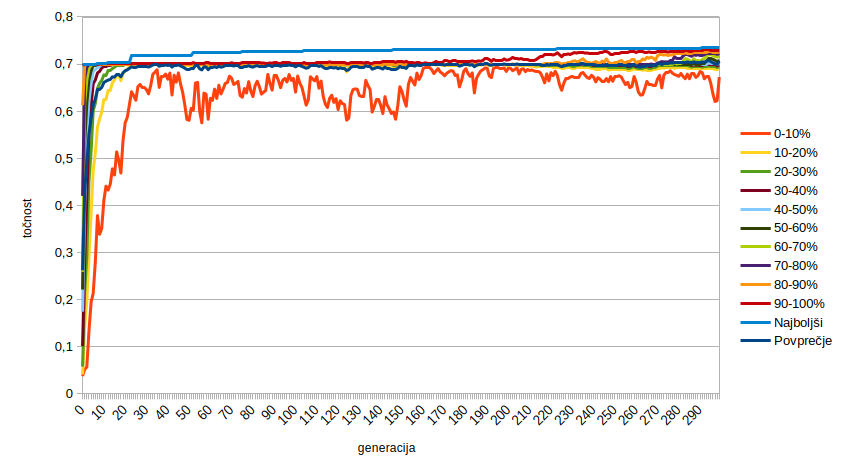
\includegraphics[width=13cm]{car/3/acc}
    \end{center}
    \caption{Graf točnosti populacije najboljšega agenta tretjega nabora skozi generacije.}
    \label{fig:car_acc_3}
\end{figure}

\begin{figure}[H]
    \begin{center}
        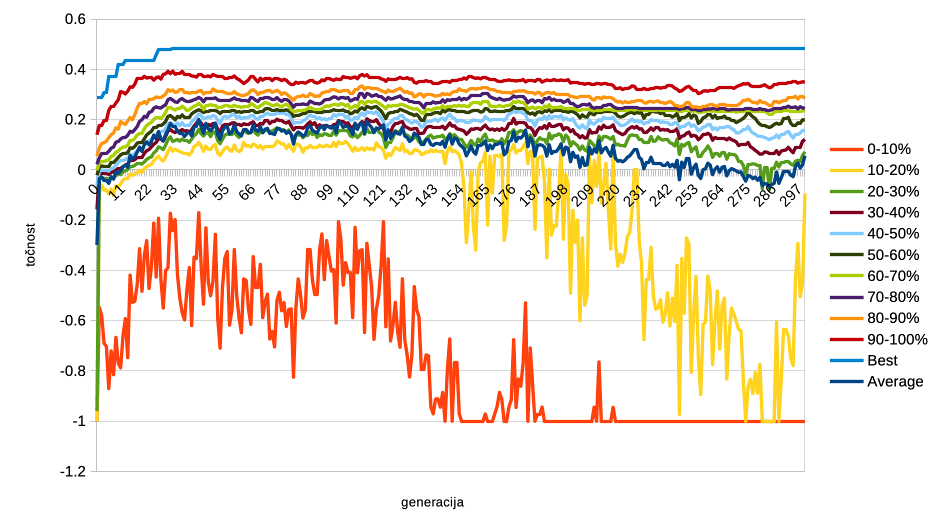
\includegraphics[width=13cm]{car/3/mcc}
    \end{center}
    \caption{Graf MCC populacije najboljšega agenta tretjega nabora skozi generacije.}
    \label{fig:car_mcc_3}
\end{figure}

\begin{figure}[H]
    \begin{center}
        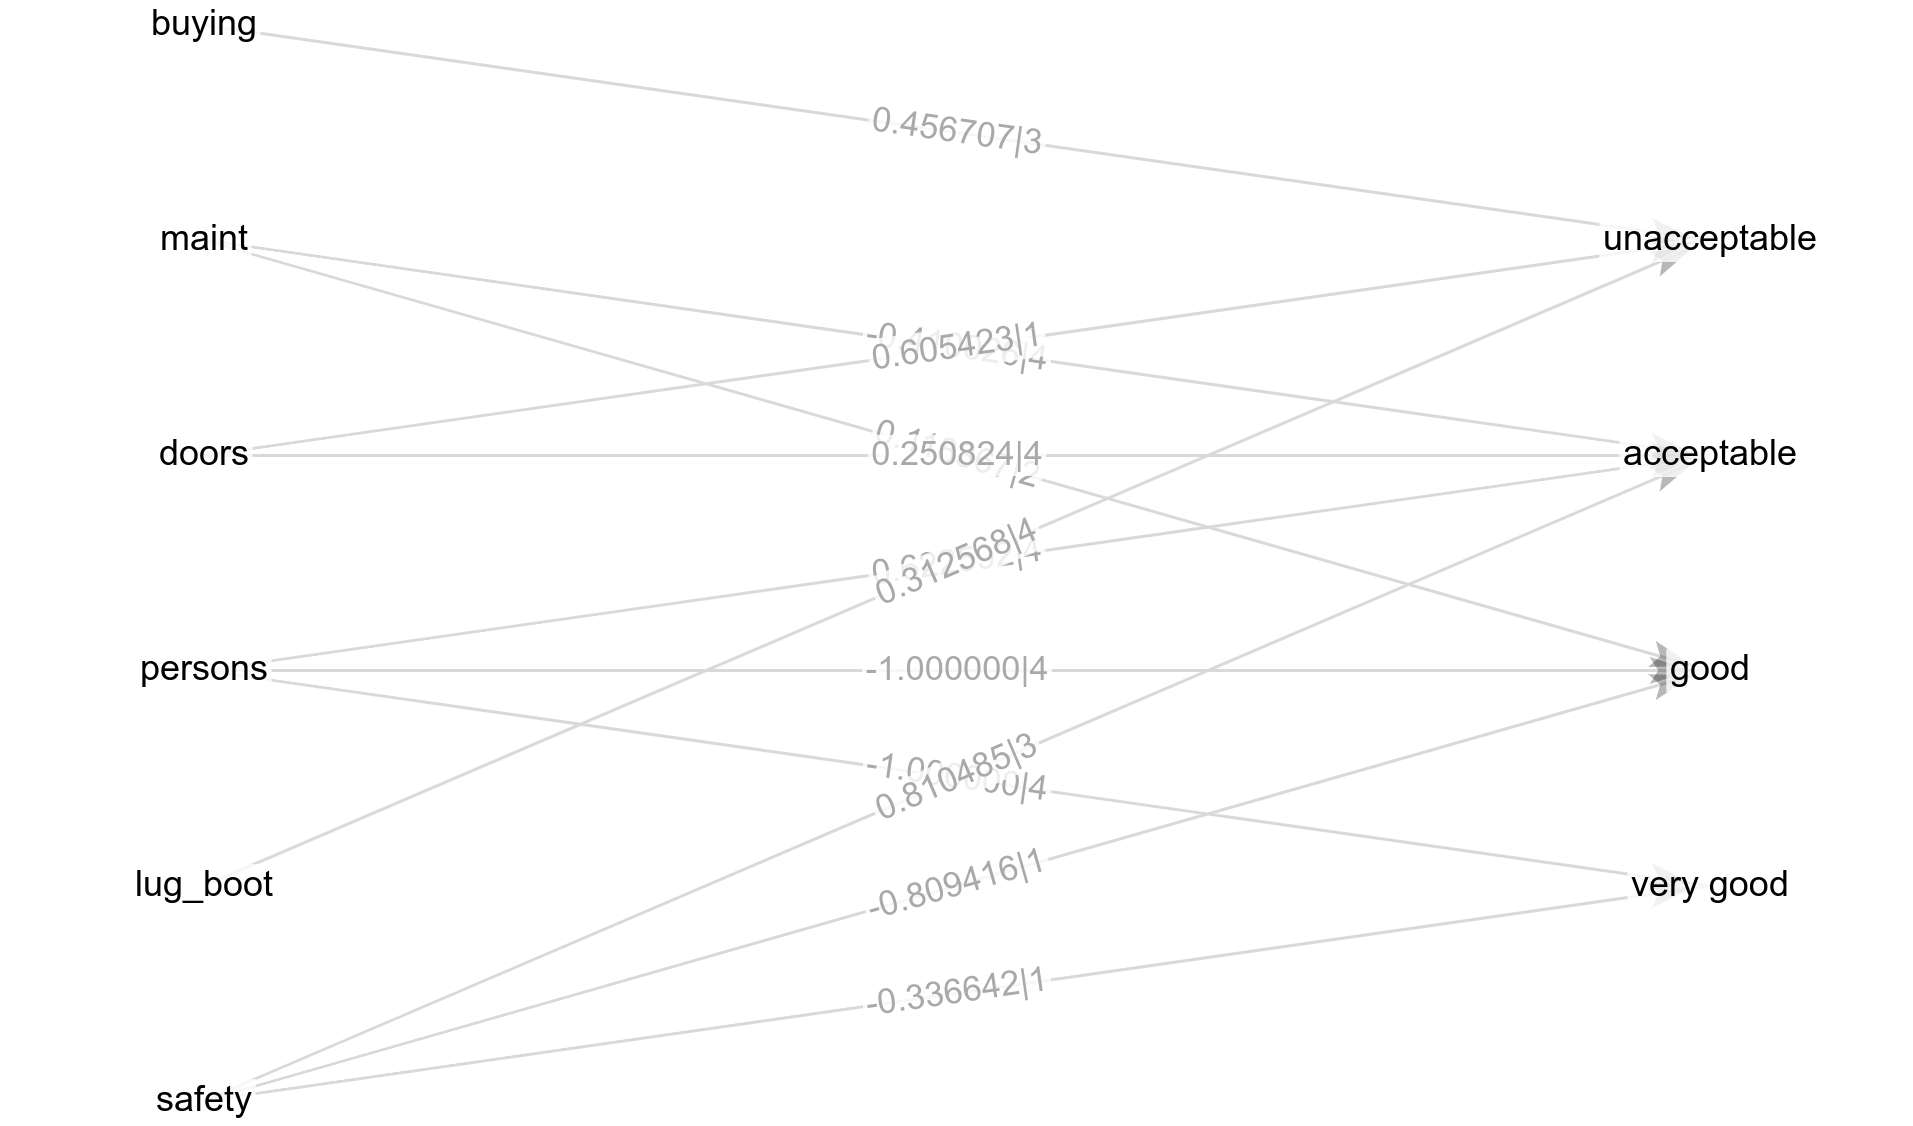
\includegraphics[width=13cm]{car/3/acc_g}
    \end{center}
    \caption{Vizualizacija najbolj točnega agenta tretjega nabora. Vsebuje 15 globokih vozlišč in 64 povezav.}
    \label{fig:car_acc_3_g}
\end{figure}

\begin{figure}[H]
    \begin{center}
        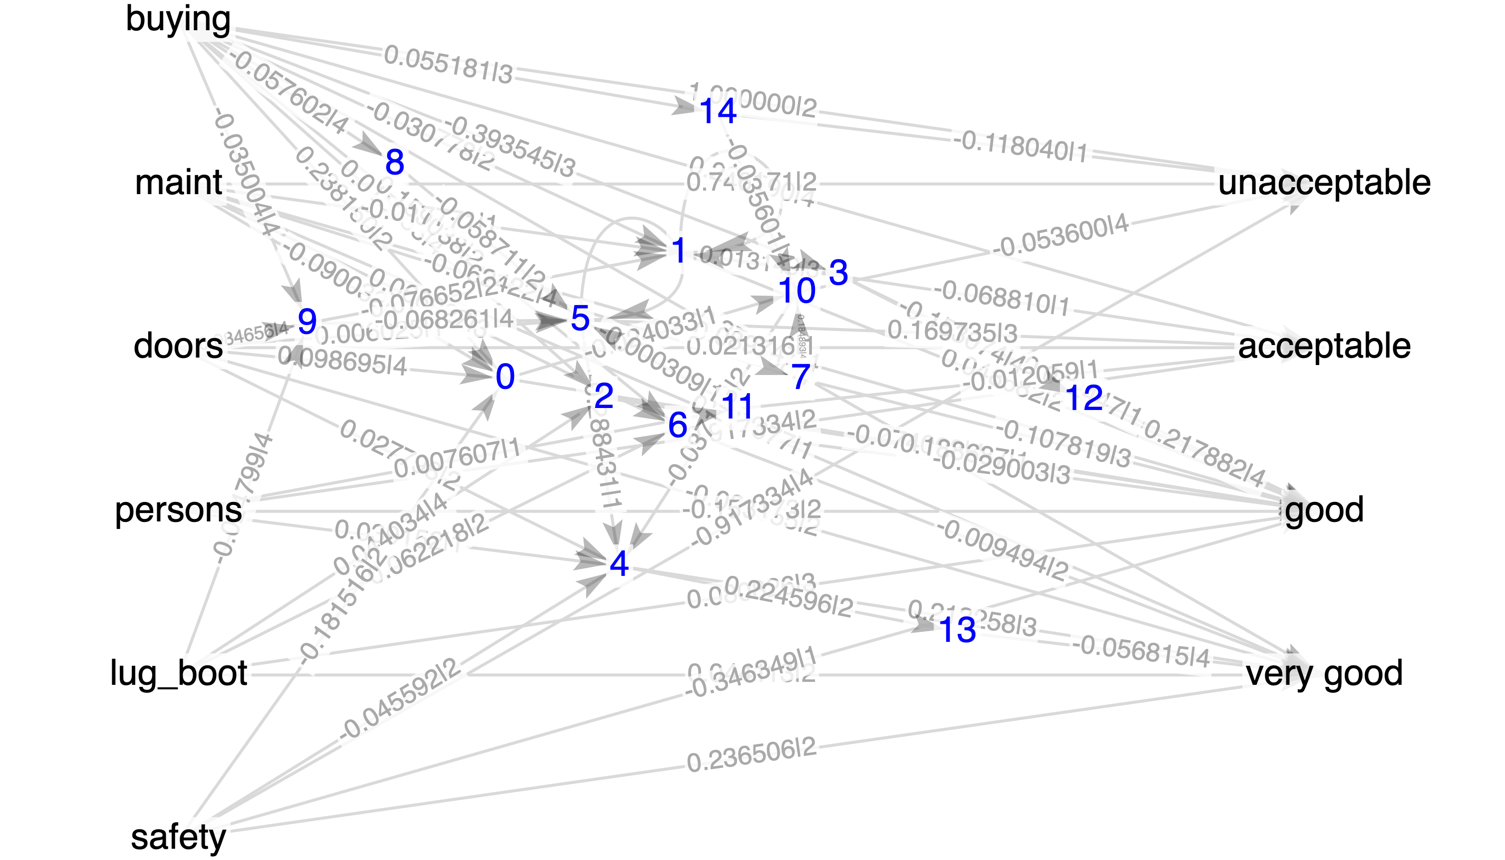
\includegraphics[width=13cm]{car/3/mcc_g}
    \end{center}
    \caption{Vizualizacija agenta z največjim MCC drugega nabora. Vsebuje 15 globokih vozlišč in 67 povezav.}
    \label{fig:car_mcc_3_g}
\end{figure}


\subsection{Shuttle}\label{subsec:statlog_test}
%% arrowLength=10
%% linkWidth=3
%% input fy=50*node.pos
%% output fx=550
%% output fy=50*node.pos+25
%% MAX_FONT_SIZE=8
\begin{table}[H]
    \caption{Nabori inicializacijskih parametrov poganjanja na množici Shuttle.}
    \begin{center}
        \begin{tabular}{||l c c c||}
            \hline
            & 1        & 2        & 3 \\ [0.5ex]
            \hline
            velikost populacije               & 200      & 250      & 350      \\
            \hline
            največje število globokih vozlišč & 15       & 20       & 40       \\
            \hline
            največje število povezav          & 30       & 50       & 100      \\
            \hline
            največje število prečkanj         & 2        & 3        & 4        \\
            \hline
            delež mutiranih potomcev          & 10\%     & 10\%     & 10\%     \\
            \hline
            prispevek vozlišč                 & -0.00001 & -0.00001 & -0.00001 \\
            \hline
            prispevek povezav                 & -0.00001 & -0.00001 & -0.00001 \\
            \hline
            število generacij                 & 200      & 250      & 300      \\
            \hline
        \end{tabular}
    \end{center}
    \label{tab:param_statlog}
\end{table}

\subsubsection{Prvi nabor}
%% branch shuttle
%% 200 15 30 2 true 0.1 100 true -0.00001 -0.00001 200 ACC


%\cleardoublepage
%\addcontentsline{toc}{chapter}{Literatura}

%\printbibliography[heading=bibintoc,type=article,title={Članki v revijah}]

%\printbibliography[heading=bibintoc,type=inproceedings,title={Članki v zbornikih}]

%\printbibliography[heading=bibintoc,type=incollection,title={Poglavja v knjigah}]

\printbibliography[heading=bibintoc,title={Celotna literatura}]